\documentclass[11pt]{article}

\usepackage[margin=0.8in]{geometry}
\usepackage{graphicx}
\usepackage{booktabs}
\usepackage{longtable}
\usepackage{array}
\usepackage{siunitx}
\usepackage{amsmath}
\usepackage{amssymb}
\usepackage{caption}
\usepackage{subcaption}
\usepackage{float}
\usepackage{xcolor}
\usepackage{placeins}
\usepackage[hidelinks]{hyperref}
\hypersetup{pdftitle={Structural Sizing and Weight Optimisation of a NACA 2412 Two-Cell Wing Box}, pdfauthor={Ignacio Garc\'ia Pere\~na}}

\sisetup{
  detect-all
}

\graphicspath{{../outputs/figures/}}

\newcommand{\finalweight}{449.4477}
\newcommand{\projecttitle}{Structural Sizing and Weight Optimisation of a NACA 2412 Two-Cell Wing Box}

\title{\projecttitle}
\author{Ignacio Garc\'ia Pere\~na}
\date{June 2026}

\begin{document}
\maketitle

\begin{abstract}
This report presents the structural sizing of a NACA 2412 wing box for a rectangular-wing, utility-category light aircraft, carried out as a personal engineering project. The workflow connects aircraft-level flight-envelope loads to local structural checks by generating the critical aerodynamic load cases, converting them into spanwise shear, bending, and torsional distributions, and evaluating the resulting stresses and stability margins along the wing. The structural model includes a two-cell wing-box idealisation with skins, spar webs, spar caps, stringers, and a geometric rib-weight model. A four-stage adaptive Monte Carlo optimisation selected the final design after evaluating 20,000 candidate designs across 13 design variables. The selected candidate is the lightest passing design found across all stages, with a reported structural weight of 449.45 lb including ribs and excluding miscellaneous detailed-design items. The design passes the implemented numerical checks for ultimate-load yield, Euler column buckling, divergence, and combined panel buckling.
\end{abstract}

\tableofcontents
\newpage

\section{Introduction and Design Objective}

The design objective was to minimise wing-box structural weight while satisfying the implemented structural screening checks. The study connects airfoil-level aerodynamic data, aircraft geometry, flight-envelope loads, and local structural checks in one sizing workflow. The analysis starts from the NACA 2412 polar data and the aircraft design inputs, builds the manoeuvre and gust envelope, converts the critical flight conditions into spanwise load distributions, and then carries those distributions into the structural sizing and optimisation model. The structural model captures the primary load paths in a two-cell NACA 2412 wing box: spar caps and stringers carry the main bending loads, thin-walled skins and spar webs carry shear and torsion, and rib spacing controls bay stability. The final optimisation considered spar locations, skin and web thicknesses, stringer counts, rib spacing, stringer section selection, and spar-cap section selection. The numerical pass/fail checks include ultimate-load von Mises yield screening, Euler column buckling, divergence, and panel buckling with bay-averaged combined loading. Table~\ref{tab:projectdata} lists the aircraft data that define the study, and Table~\ref{tab:finalcandidate} gives a snapshot of the final result.


\begin{table}[H]
\centering
\caption{Aircraft geometry and flight data used as design inputs.}
\label{tab:projectdata}
\begin{tabular}{lll}
\toprule
Category & Quantity & Value \\
\midrule
Geometry & Airfoil & NACA 2412 \\
Geometry & Planform & Rectangular \\
Geometry & Chord & 5 ft / 60 in \\
Geometry & Semispan & 17 ft / 204 in \\
Geometry & Full span & 34 ft \\
Geometry & Wing area & 170 ft$^2$ \\
Geometry & Aspect ratio & 6.8 \\
Weights & Maximum weight, $W_{\max}$ & 3200 lb \\
Weights & Minimum weight, $W_{\min}$ & 1900 lb \\
Speeds & Cruise speed, $V_C$ & 230 mph \\
Speeds & Dive speed, $V_D$ & 270 mph \\
Envelope & Utility positive load factor & +4.4 \\
Envelope & Utility negative load factor & -1.76 \\
Gust & Gust velocity at $V_C$ & 50 ft/s \\
Gust & Gust velocity at $V_D$ & 25 ft/s \\
\bottomrule
\end{tabular}
\end{table}

\begin{table}[H]
\centering
\caption{Final result snapshot.}
\label{tab:finalcandidate}
\begin{tabular}{ll}
\toprule
Quantity & Value \\
\midrule
Final reported weight & \SI{449.45}{lb} \\
Search size & 20,000 candidate designs \\
Selected stage & Stage 2 global best \\
Overall status & Pass \\
\bottomrule
\end{tabular}
\end{table}

\begin{table}[H]
\centering
\caption{Analysis workflow and data flow.}
\label{tab:workflow}
\small
\begin{tabular}{>{\raggedright\arraybackslash}p{0.21\linewidth}>{\raggedright\arraybackslash}p{0.43\linewidth}>{\raggedright\arraybackslash}p{0.27\linewidth}}
\toprule
Block & Method / data handled & Output to next step \\
\midrule
Design inputs & Geometry, utility-category limits, speeds, weights, and airfoil data & Basic flight and geometry constants \\
Aerodynamic polar processing & NACA 2412 coefficients, finite-wing correction, and force transformation & $C_N$, $C_X$, and $C_M$ for critical flight points \\
Flight-envelope and gust analysis & Manoeuvre envelope, gust lines, and critical condition selection & High-angle, limit-angle, and gust load cases \\
Spanwise load generation & Distributed $q_z$, $q_x$, and pitching-moment loads with tip-inward integration & $V_x$, $V_z$, $M_x$, $M_z$, and $M_y$ along the semispan \\
Wing-box geometry setup & Spars, skins, webs, stringers, spar caps, and ribs & Structural geometry and panel definitions \\
Section idealisation & Boom/panel idealisation, centroid, inertias, and shear center & Stress and shear-flow coefficients \\
Spanwise structural evaluation & Loads interpolated at rib stations and panel bays & Yield, column, panel buckling, and divergence ratios \\
Weight model & Component weights plus geometric rib model & Total analysed structural weight \\
Manual verification sweeps & Sanity checks on range choices and response trends & Feasible optimisation ranges \\
Adaptive Monte Carlo optimisation & Four-stage random search with elite-based range refinement & Lightest passing final design found \\
\bottomrule
\end{tabular}
\end{table}


\section{Aerodynamic Loading and Flight Envelope}

The final structural checks use the aerodynamic load cases and spanwise load distributions produced by the flight-envelope and aerodynamic load analysis described in this section. The aircraft is sized to the utility-category requirements of 14 CFR Part 23~\cite{far23} with a rectangular NACA 2412 wing planform, chord $c=\SI{60}{in}$, and semispan $b/2=\SI{204}{in}$. The load-generation workflow starts with XFOIL 6.99 polar extraction, applies a finite-wing correction, transforms lift and drag into body-axis force coefficients, builds the manoeuvre and gust envelope, selects critical load cases, distributes those loads along the semispan, and integrates them into structural shear, bending, and torsion inputs.

XFOIL 6.99~\cite{xfoil} generated the NACA 2412 section polar at $Re=5.0\times10^6$, Mach 0, and $N_{\mathrm{crit}}=9$ over $\alpha=-23^\circ$ to $25^\circ$. The extracted high-angle points included $C_{l,\max}=1.8523$ at $\alpha=19.5^\circ$ with $C_D=0.04610$, and $C_{l,\min}=-1.6245$ at $\alpha=-19^\circ$ with $C_D=0.02987$. These two-dimensional values provide the starting point for the finite-wing correction and load-envelope calculation. The two-dimensional lift coefficient was converted to a finite-wing coefficient using
\begin{equation}
  C_L = \frac{c_l}{1 + c_l/(\pi ARe)},
\end{equation}
with aspect ratio $AR=6.8$ and Oswald efficiency factor $e=0.8$.

The positive high-angle structural case applies a 25 percent margin to the high-angle lift condition, since this point drives a conservative angle-of-attack load case near the edge of the polar data. The resulting case uses $\alpha_{\mathrm{PHAA}}=24.375^\circ$, $C_L=2.0890$, $C_D=0.158795$, $C_N=1.9683$, and $C_X=-0.7175$. The pitching-moment coefficient for this case, $C_M=-0.0528$, is a fixed input of the load-generation model.

The flight envelope defines the positive and negative manoeuvre and gust cases used to identify critical load states, following the manoeuvring and gust-envelope definitions of 14 CFR 23.333, 23.337 and 23.341~\cite{far23}. The manoeuvre load factor was evaluated from
\begin{equation}
  n = \frac{\frac{1}{2}\rho V^2 S C_N}{W},
\end{equation}
where the body-axis transformation converts lift and drag into the normal-force coefficient
\begin{equation}
  C_N = C_L \cos\alpha + C_D \sin\alpha,
  \qquad
  C_X = C_D \cos\alpha - C_L \sin\alpha .
\end{equation}
The gust increments were evaluated using
\begin{equation}
  \Delta n =
  \frac{\rho S C_{L_\alpha} V U_{de} k}{2W},
\end{equation}
where $U_{de}$ is the design gust velocity and $k$ is the gust alleviation factor based on the mass ratio $\mu$, $k = 0.88\mu/(5.3+\mu)$~\cite{far23}.

\begin{table}[H]
\centering
\caption{Gust-envelope constants and resulting gust load factors.}
\label{tab:gustconstants}
\begin{tabular}{ll}
\toprule
Quantity & Value \\
\midrule
$C_{L_\alpha,\mathrm{3D}}$ & \SI{4.5942}{rad^{-1}} \\
Mass ratio, $\mu$ & 12.708 \\
Gust alleviation factor, $k$ & 0.6210 \\
$\Delta n$ at $V_C$ & 5.1236 \\
$\Delta n$ at $V_D$ & 3.0073 \\
Positive gust at $V_C$ & 6.1236 \\
Negative gust at $V_C$ & -4.1236 \\
Positive gust at $V_D$ & 4.0073 \\
Negative gust at $V_D$ & -2.0073 \\
\bottomrule
\end{tabular}
\end{table}

The nine critical cases combine five manoeuvre-envelope points and four gust points. The case names give the sign and the condition: PHAA/NHAA are the positive/negative high-angle-of-attack cases, PLAA/NLAA the positive/negative low-angle-of-attack cases, and PG/NG the positive/negative gust cases, with the suffix VC or VD for the speed. The stall lines meet the limit load factors at the manoeuvring speeds $V_{A\pm}=\sqrt{2|n|W/(\rho S|C_N|)}$, which give $V_{A+}=\SI{128.2}{mph}$ for the PHAA corner ($n=4.4$, $W_{\max}$) and $V_{A-}=\SI{73.8}{mph}$ for the NHAA corner ($n=-1.76$, $W_{\min}$). The other three envelope corners are PLAA ($V_D$, $n=4.4$), NLAA\_VC ($V_C$, $n=-1.76$) and NLAA\_VD ($V_D$, $n=-1.0$). PHAA and PLAA use $W_{\max}=\SI{3200}{lb}$; the other seven cases use $W_{\min}=\SI{1900}{lb}$. Table~\ref{tab:loadcases} lists the nine cases.

\begin{table}[H]
\centering
\caption{Critical load cases. Root loads are limit loads per semispan, before the 1.5 ultimate factor; $M_y$ is the aerodynamic pitching moment only.}
\label{tab:loadcases}
\scriptsize
\setlength{\tabcolsep}{3pt}
\begin{tabular}{lrrrrrrrrrrr}
\toprule
Case & $V$ (mph) & $n$ & $\alpha$ ($^\circ$) & $C_N$ & $C_X$ & $C_M$ & $V_z$ (lb) & $M_x$ (lb-ft) & $V_x$ (lb) & $M_z$ (lb-ft) & $M_y$ (lb-ft) \\
\midrule
PHAA & 128.2 & 4.4000 & 24.38 & 1.9683 & $-$0.7175 & $-$0.0528 & 7{,}040 & 55{,}316 & $-$2{,}566 & $-$22{,}643 & $-$944 \\
NHAA & 73.8 & $-$1.7600 & $-$19.00 & $-$1.4124 & $-$0.4547 & $-$0.0716 & $-$1{,}672 & $-$13{,}138 & $-$538 & $-$4{,}750 & $-$424 \\
PLAA & 270.0 & 4.4000 & 3.41 & 0.4438 & $-$0.0211 & $-$0.0520 & 7{,}040 & 55{,}316 & $-$334 & $-$2{,}948 & $-$4{,}124 \\
NLAA\_VC & 230.0 & $-$1.7600 & $-$3.94 & $-$0.1453 & $-$0.0039 & $-$0.0520 & $-$1{,}672 & $-$13{,}138 & $-$45 & $-$400 & $-$2{,}993 \\
NLAA\_VD & 270.0 & $-$1.0000 & $-$2.87 & $-$0.0599 & 0.0028 & $-$0.0520 & $-$950 & $-$7{,}465 & 45 & 393 & $-$4{,}124 \\
PG\_VC & 230.0 & 6.1236 & 4.19 & 0.5054 & $-$0.0315 & $-$0.0520 & 5{,}817 & 45{,}709 & $-$363 & $-$3{,}201 & $-$2{,}993 \\
NG\_VC & 230.0 & $-$4.1236 & $-$6.39 & $-$0.3403 & $-$0.0313 & $-$0.0520 & $-$3{,}917 & $-$30{,}780 & $-$360 & $-$3{,}175 & $-$2{,}993 \\
PG\_VD & 270.0 & 4.0073 & 0.86 & 0.2400 & 0.0017 & $-$0.0520 & 3{,}807 & 29{,}913 & 27 & 242 & $-$4{,}124 \\
NG\_VD & 270.0 & $-$2.0073 & $-$3.63 & $-$0.1202 & $-$0.0016 & $-$0.0520 & $-$1{,}907 & $-$14{,}984 & $-$26 & $-$228 & $-$4{,}124 \\
\bottomrule
\end{tabular}
\end{table}

For each load case, lift, drag, and aerodynamic pitching moment are decomposed into semi-wing root loads $F_z$, $F_x$, and $M_y$. The semi-wing vertical load $F_z/2$ is distributed along the semispan with the average of a uniform and elliptical shape,
\begin{equation}
  q_z(y) = \frac{1}{2}\left(q_{\mathrm{uniform}}(y) + q_{\mathrm{elliptic}}(y)\right),
  \qquad
  q_{\mathrm{uniform}} = \frac{F}{b/2},
  \qquad
  q_{\mathrm{elliptic}}(y) = \frac{4F}{\pi\, b/2}\sqrt{1-\left(\frac{y}{b/2}\right)^2},
\end{equation}
where $F=F_z/2$ is the semi-wing vertical load; both shapes integrate to $F$ over the semispan.
The chordwise force $F_x/2$ uses a piecewise spanwise distribution with a mild tip-effect increase: the outboard 20 percent of the semispan receives a 25 percent higher shape factor. The aerodynamic pitching moment $M_y/2$ is distributed uniformly along the semispan. Tip-inward integration then produces $V_z$, $M_x$, $V_x$, $M_z$, and aerodynamic $M_y$. Limit loads are scaled to ultimate loads with the factor of safety of 14 CFR 23.303~\cite{far23},
\begin{equation}
  L_{\mathrm{ult}} = 1.5 L_{\mathrm{limit}} .
\end{equation}
The final structural screening uses an ultimate load factor of 1.5. The vertical distributed load $q_z(y)$ is integrated from the tip inward to obtain
\begin{equation}
  V_z(y) = \int_y^{b/2} q_z(\eta)\,d\eta,
  \qquad
  M_x(y) = \int_y^{b/2} V_z(\eta)\,d\eta .
\end{equation}
The same tip-inward integration converts the chordwise distributed load $q_x(y)$ into $V_x(y)$ and $M_z(y)$, while the aerodynamic pitching-moment distribution provides the applied torsional moment $M_y(y)$. The generated critical-load table and spanwise-load data are the structural load inputs read by the final wing-box solver. The structural model interpolates these distributions at rib stations and scales them by the ultimate load factor of 1.5 for spanwise failure evaluation. Figure~\ref{fig:flightenvelope} shows the flight envelope used to select the critical cases.

\begin{figure}[H]
\centering
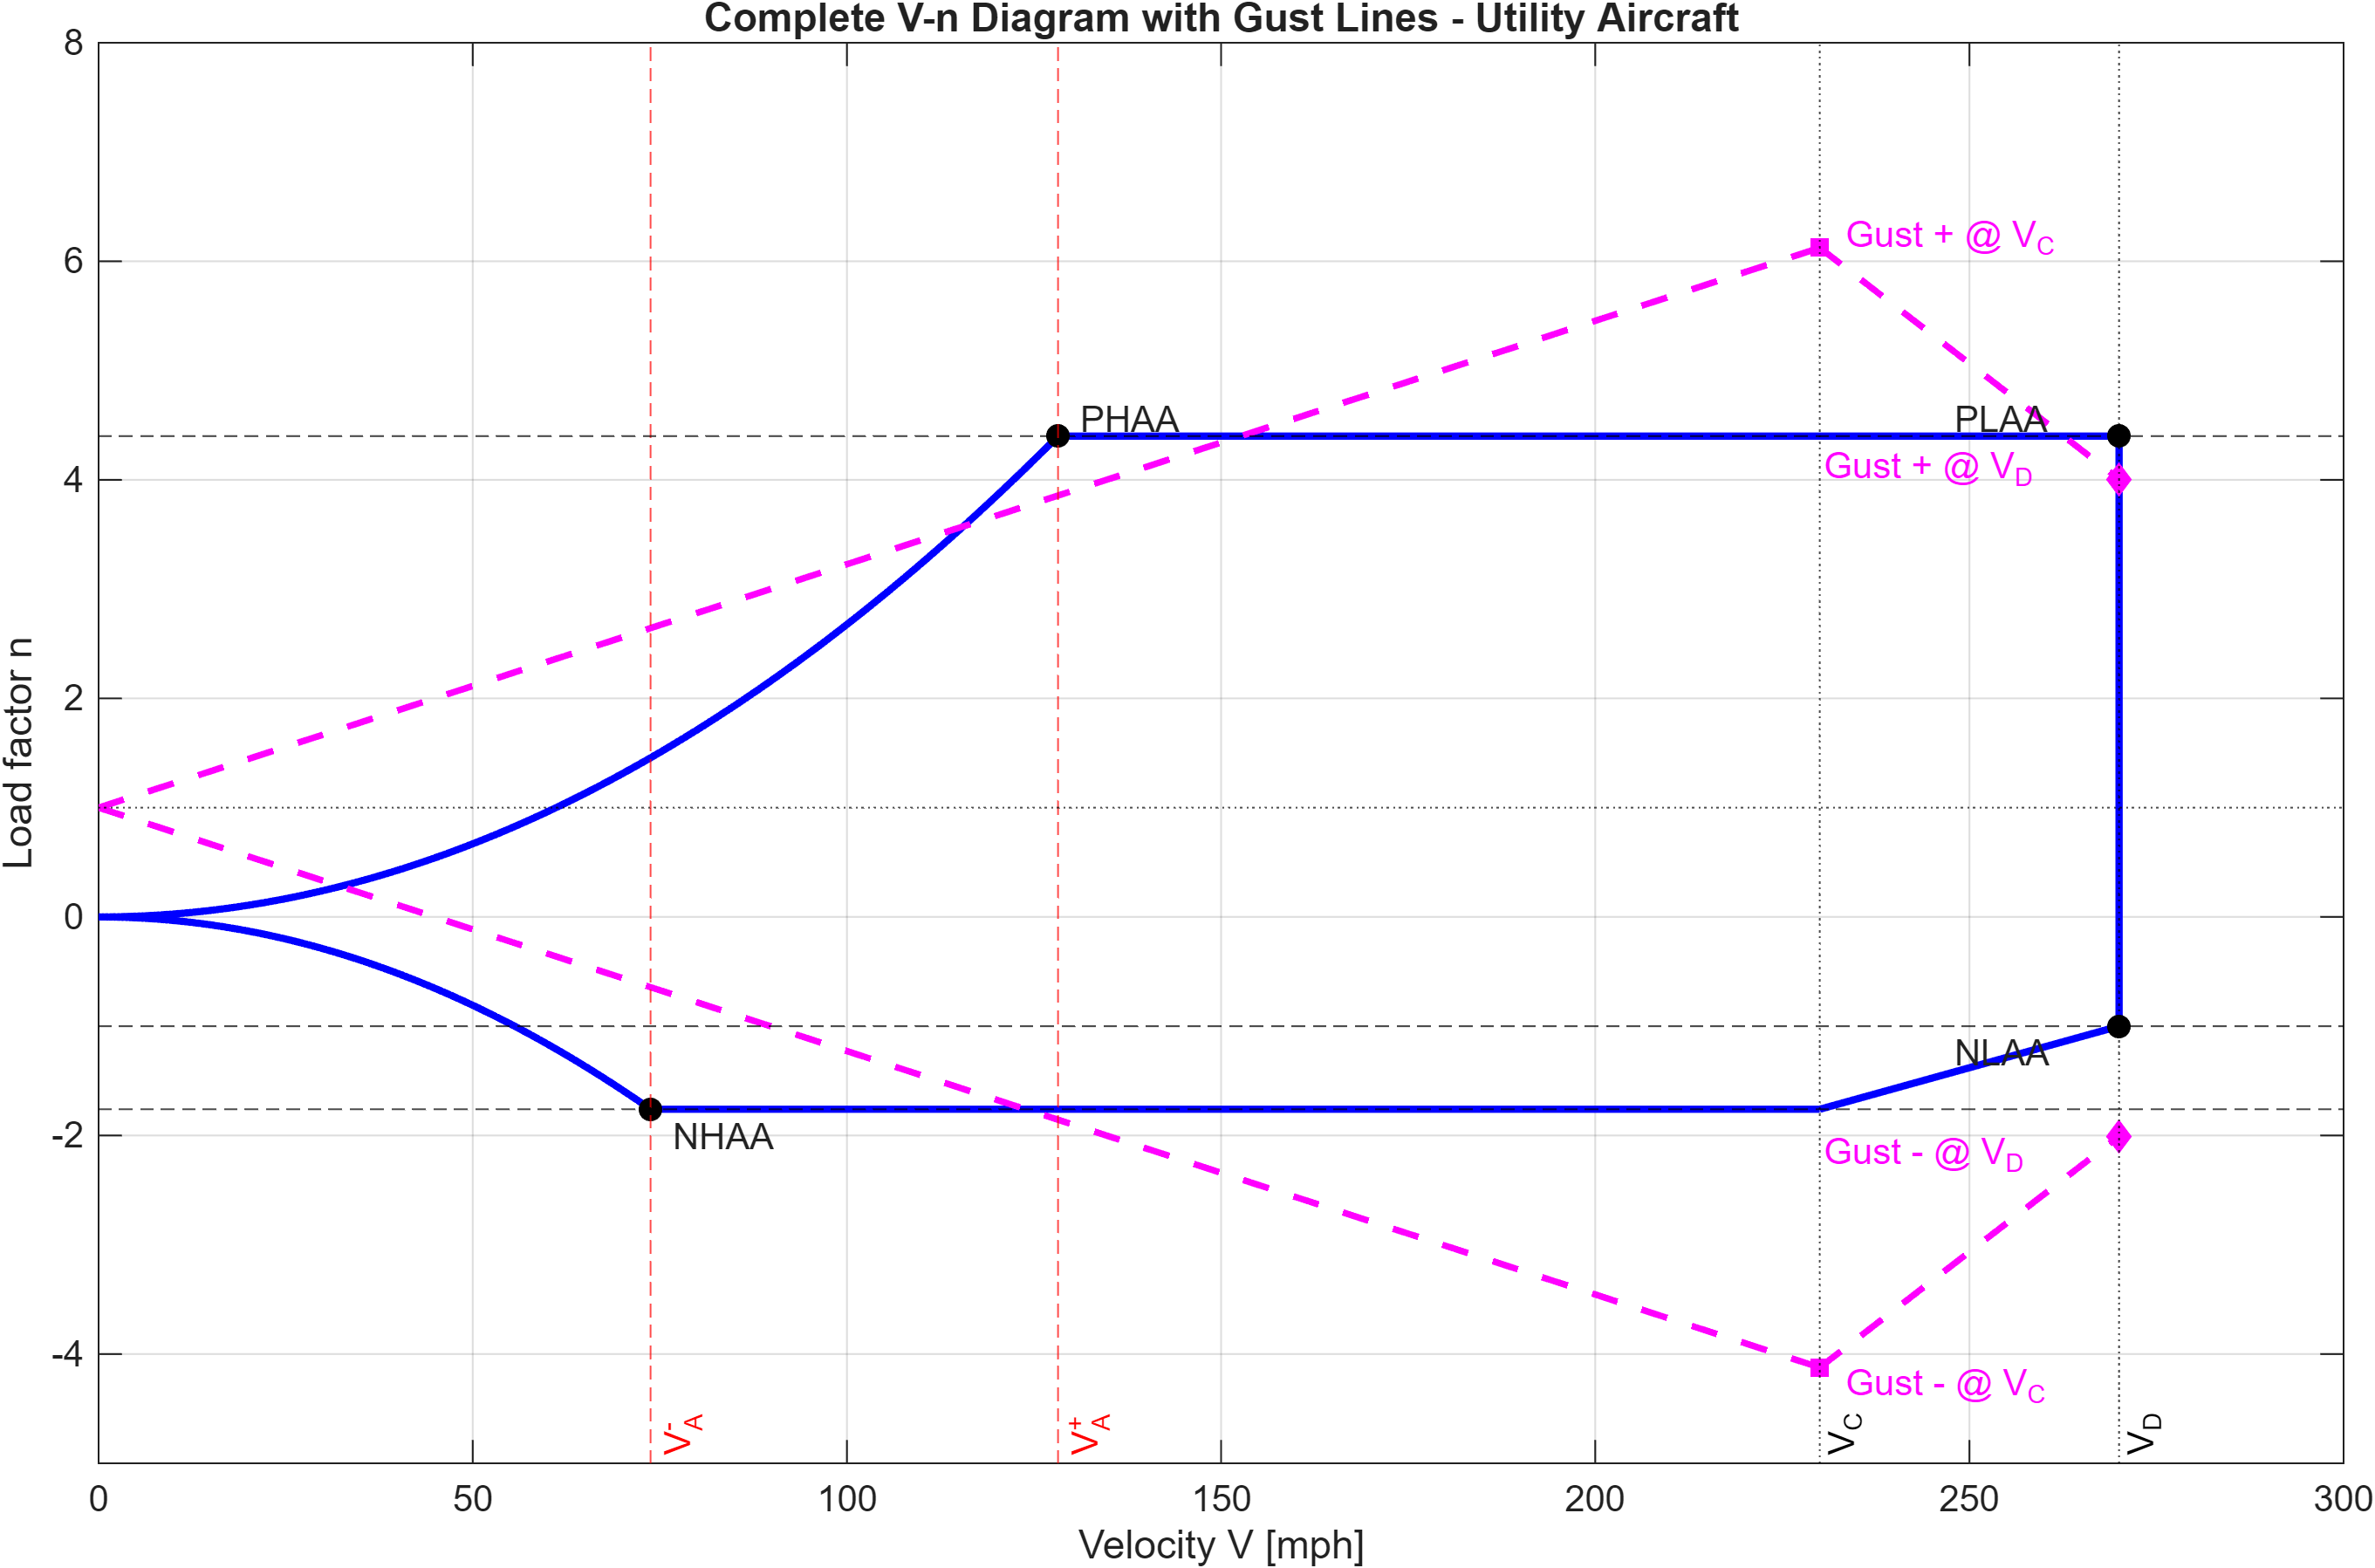
\includegraphics[width=0.80\linewidth]{final_flight_envelope.png}
\caption{Flight envelope used to define the critical aerodynamic load cases for structural sizing.}
\label{fig:flightenvelope}
\end{figure}

Figures~\ref{fig:verticalloadcases} and \ref{fig:dragtorsionloadcases} compare all nine critical load cases used by the structural solver. The vertical-load figure shows how distributed normal load $q_z(y)$ becomes vertical shear $V_z(y)$ and bending moment $M_x(y)$. The drag/torsion figure shows the chordwise and torsional inputs $q_x(y)$, $V_x(y)$, $M_z(y)$, and $M_y(y)$. Overlapping curves indicate similar or identical load components among cases, but all cases are still evaluated rather than reducing the problem to one governing case.

\begin{figure}[H]
\centering
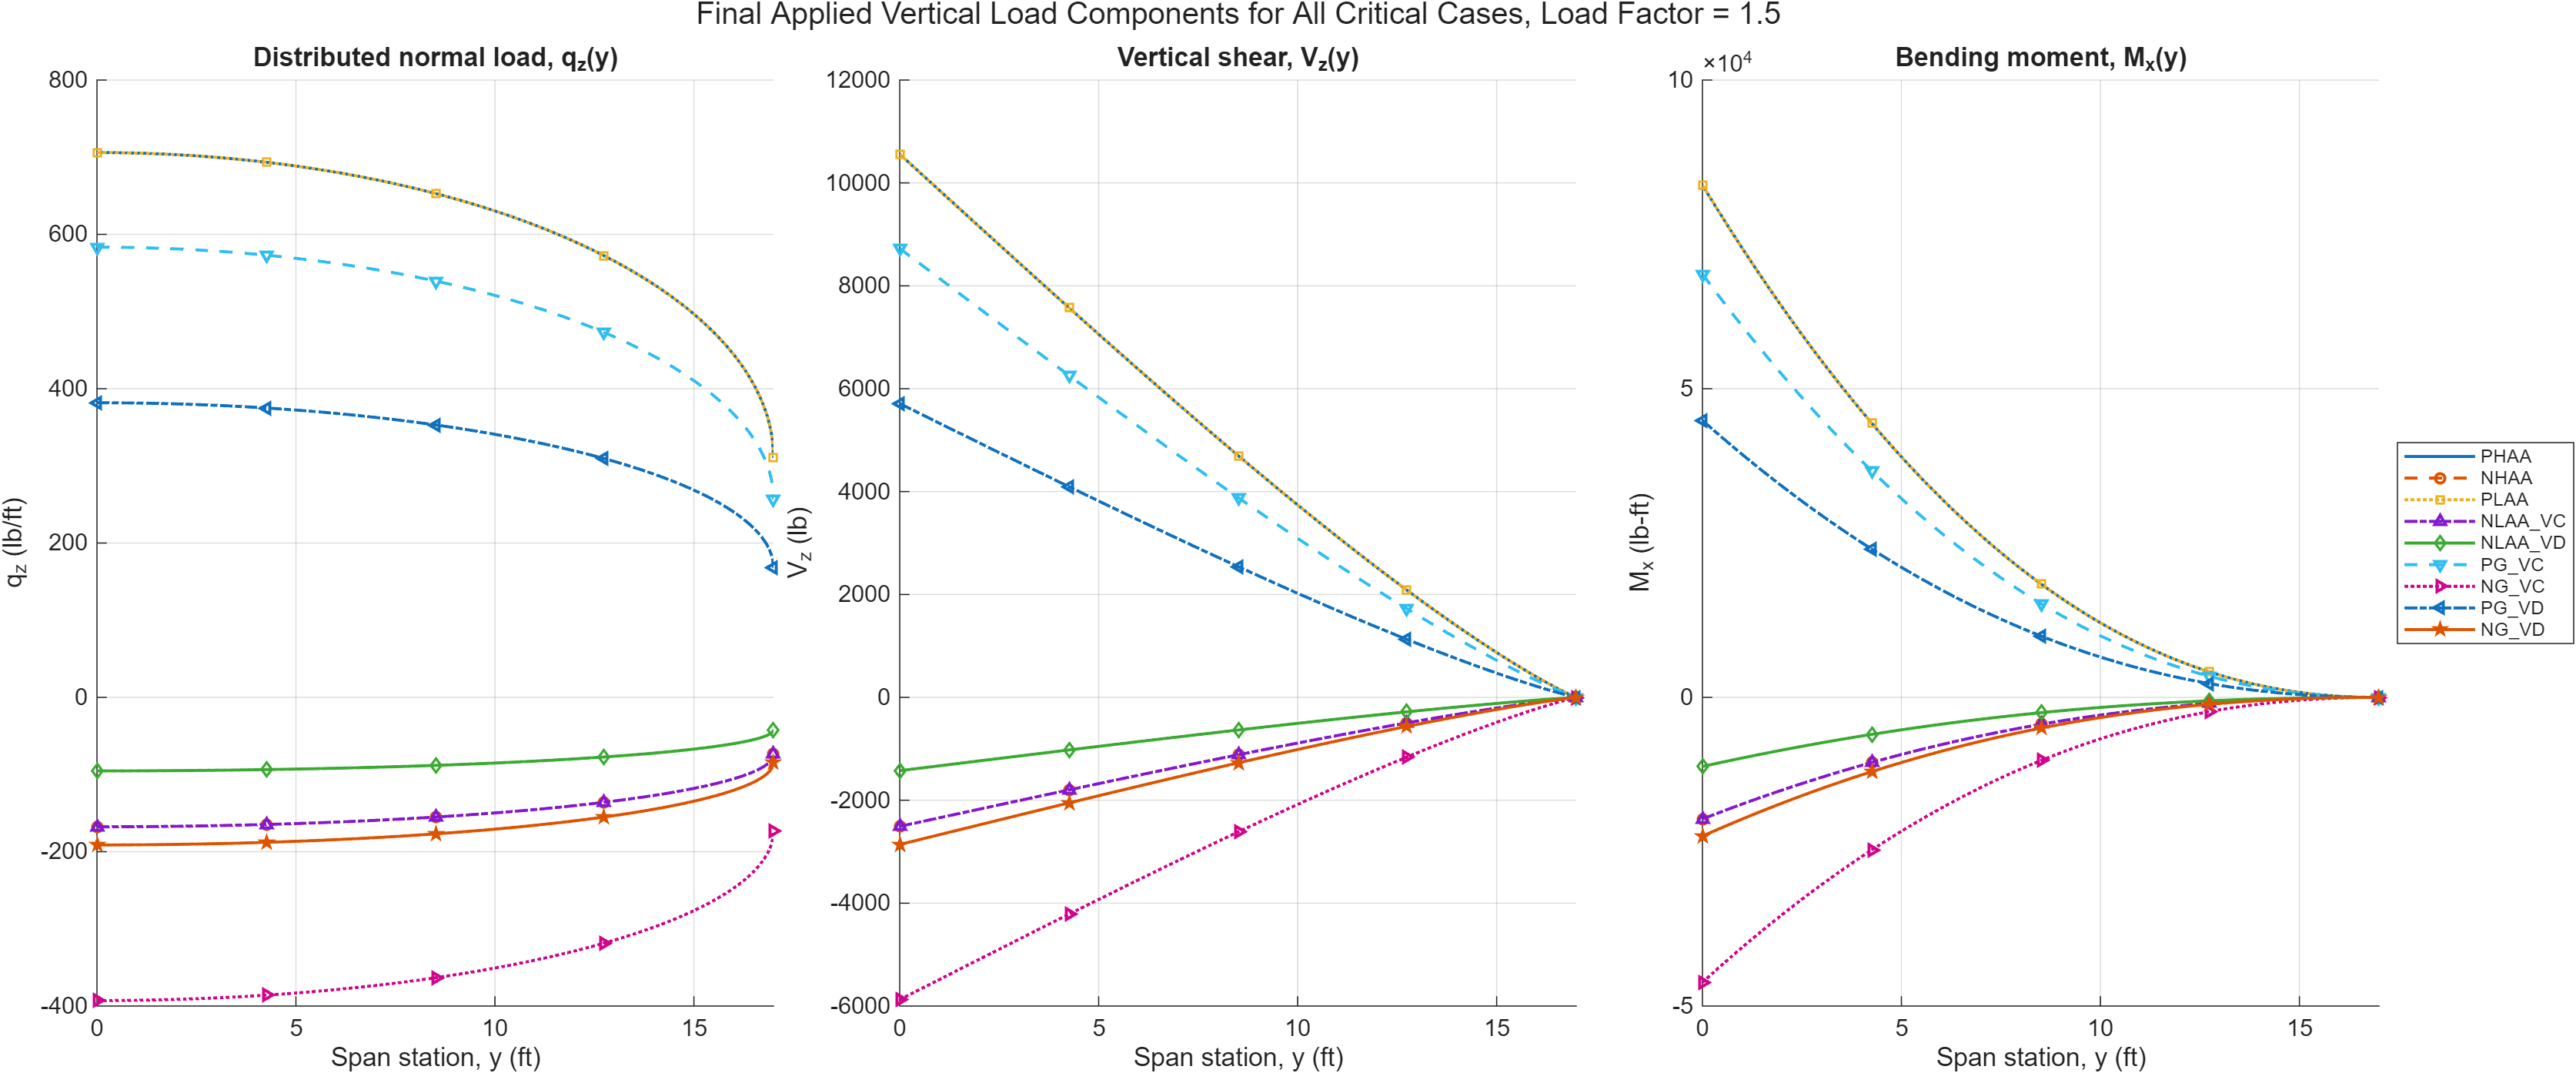
\includegraphics[width=0.98\linewidth]{final_all_cases_vertical_loads.png}
\caption{Final applied vertical load components for all nine critical cases after ultimate-load scaling. The three panels compare $q_z(y)$, $V_z(y)$, and $M_x(y)$, which are the direct structural inputs for bending stress and panel normal-stress recovery.}
\label{fig:verticalloadcases}
\end{figure}

\begin{figure}[H]
\centering
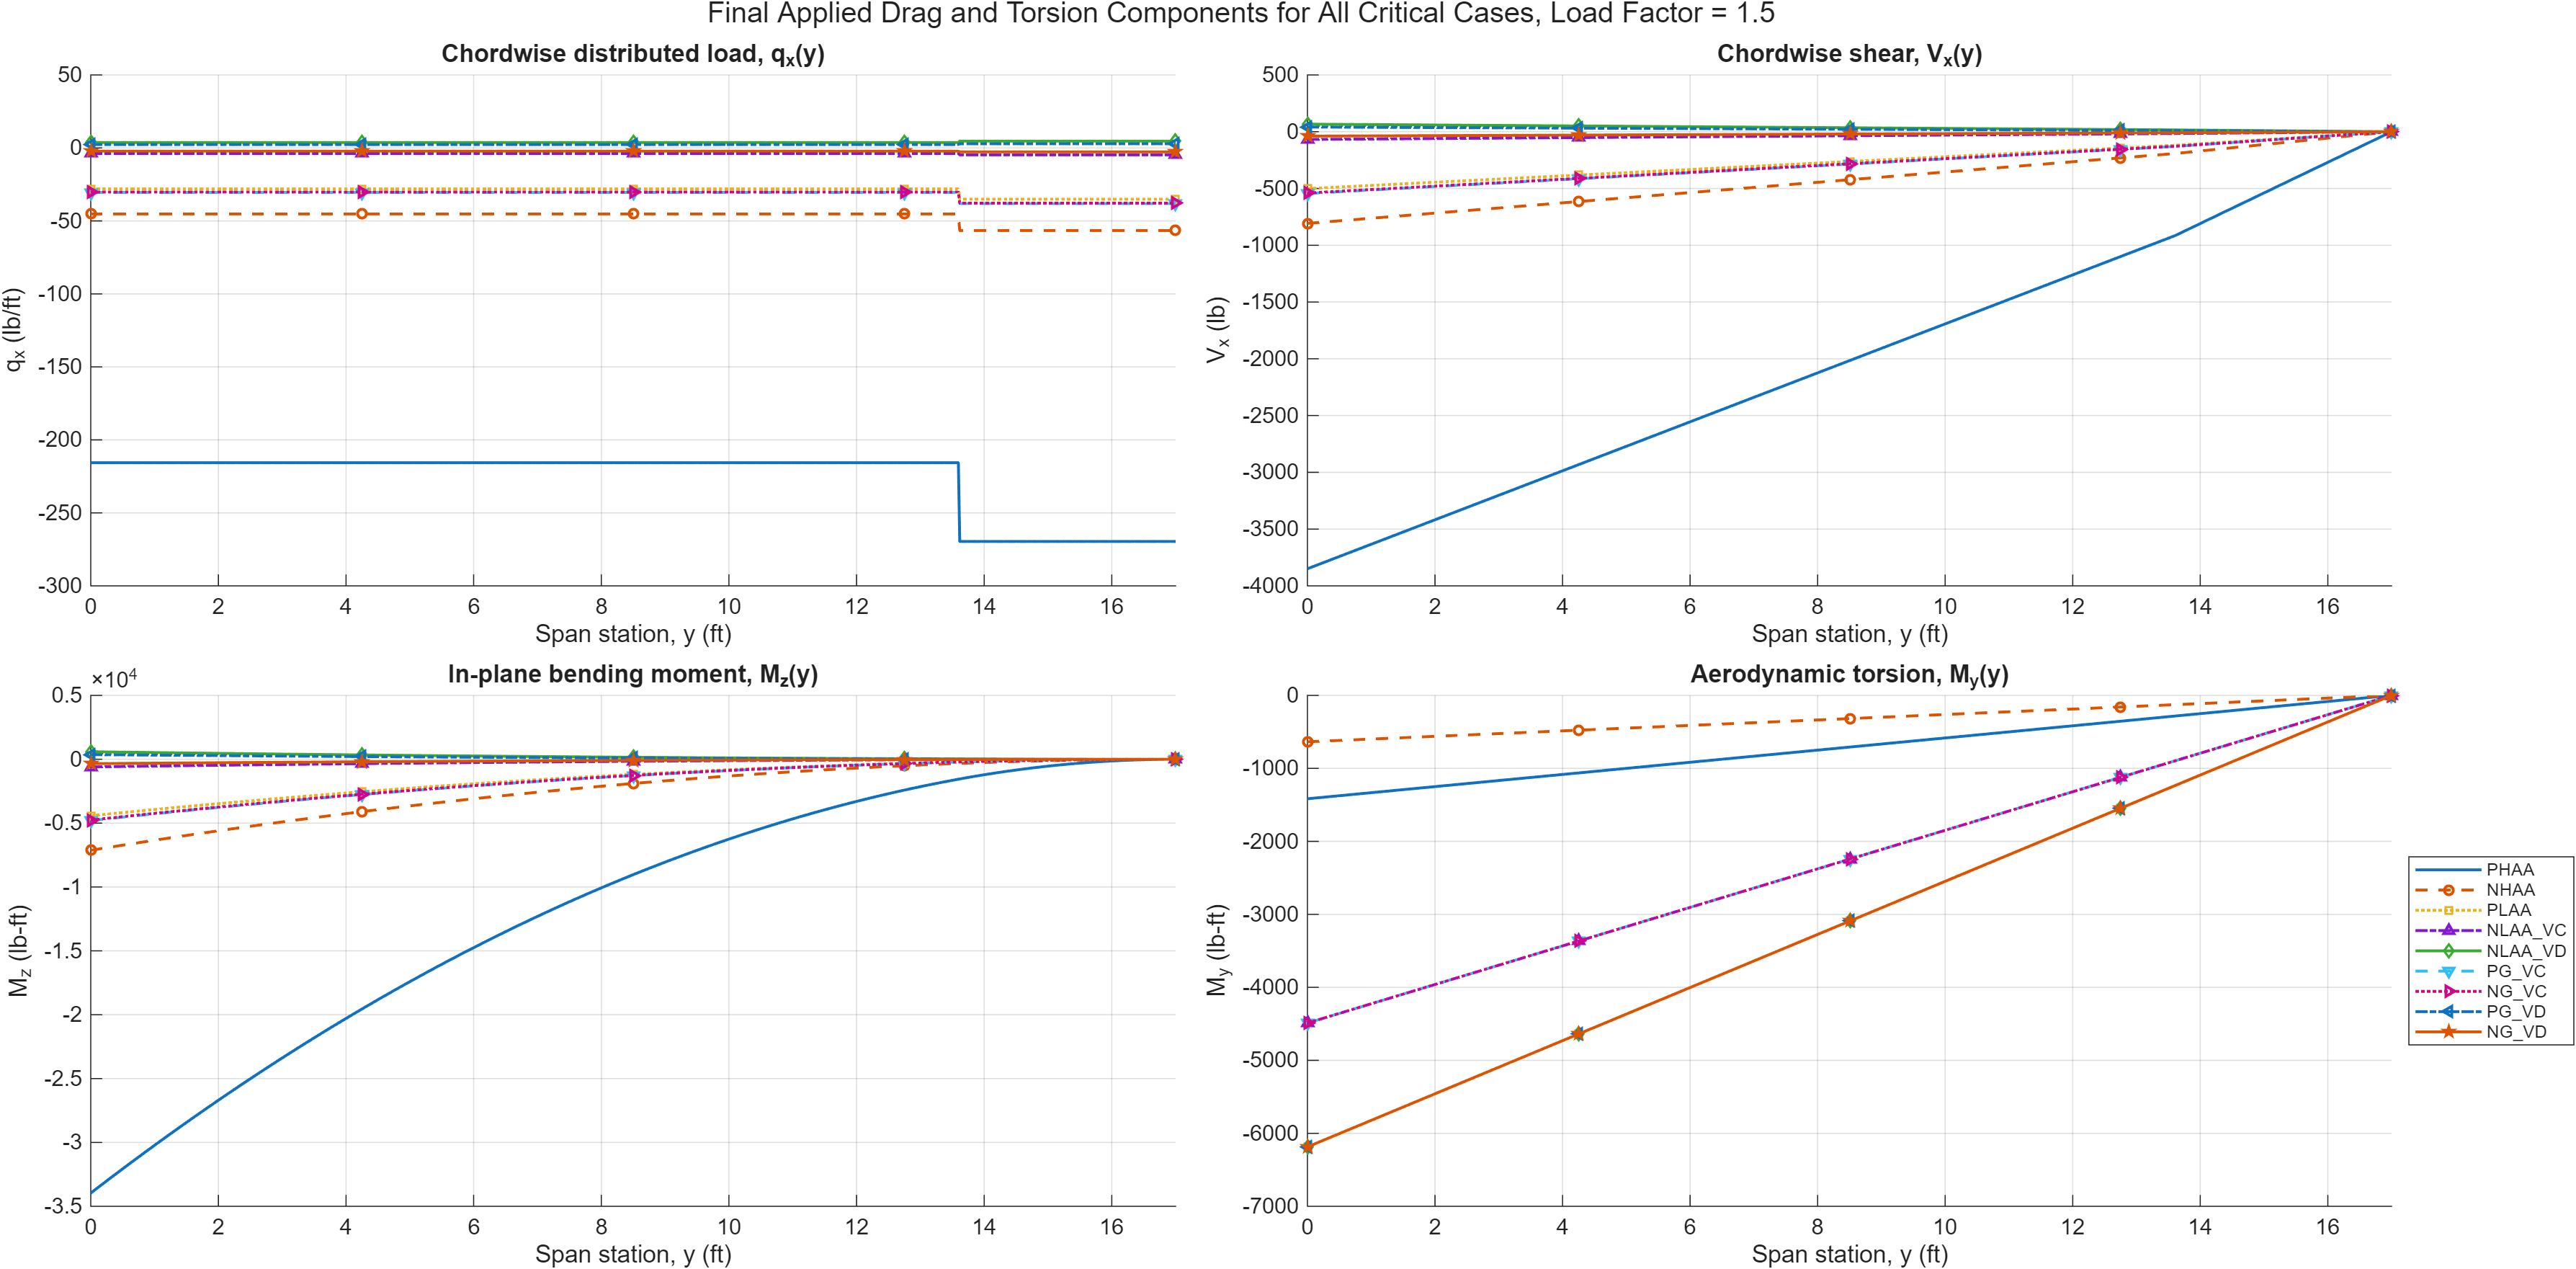
\includegraphics[width=0.98\linewidth]{final_all_cases_drag_torsion_loads.png}
\caption{Final applied drag and torsion components for all nine critical cases after ultimate-load scaling. The four panels compare $q_x(y)$, $V_x(y)$, $M_z(y)$, and aerodynamic $M_y(y)$; overlapping curves indicate cases with similar chordwise or torsional loading.}
\label{fig:dragtorsionloadcases}
\end{figure}

The load analysis includes the aerodynamic pitching moment $M_y$. The shear-flow formulation handles the vertical-load moment arm about the shear center through the unit shear-flow contribution associated with $V_z$, avoiding double-counting of shear-center torsion.

\begin{figure}[H]
\centering
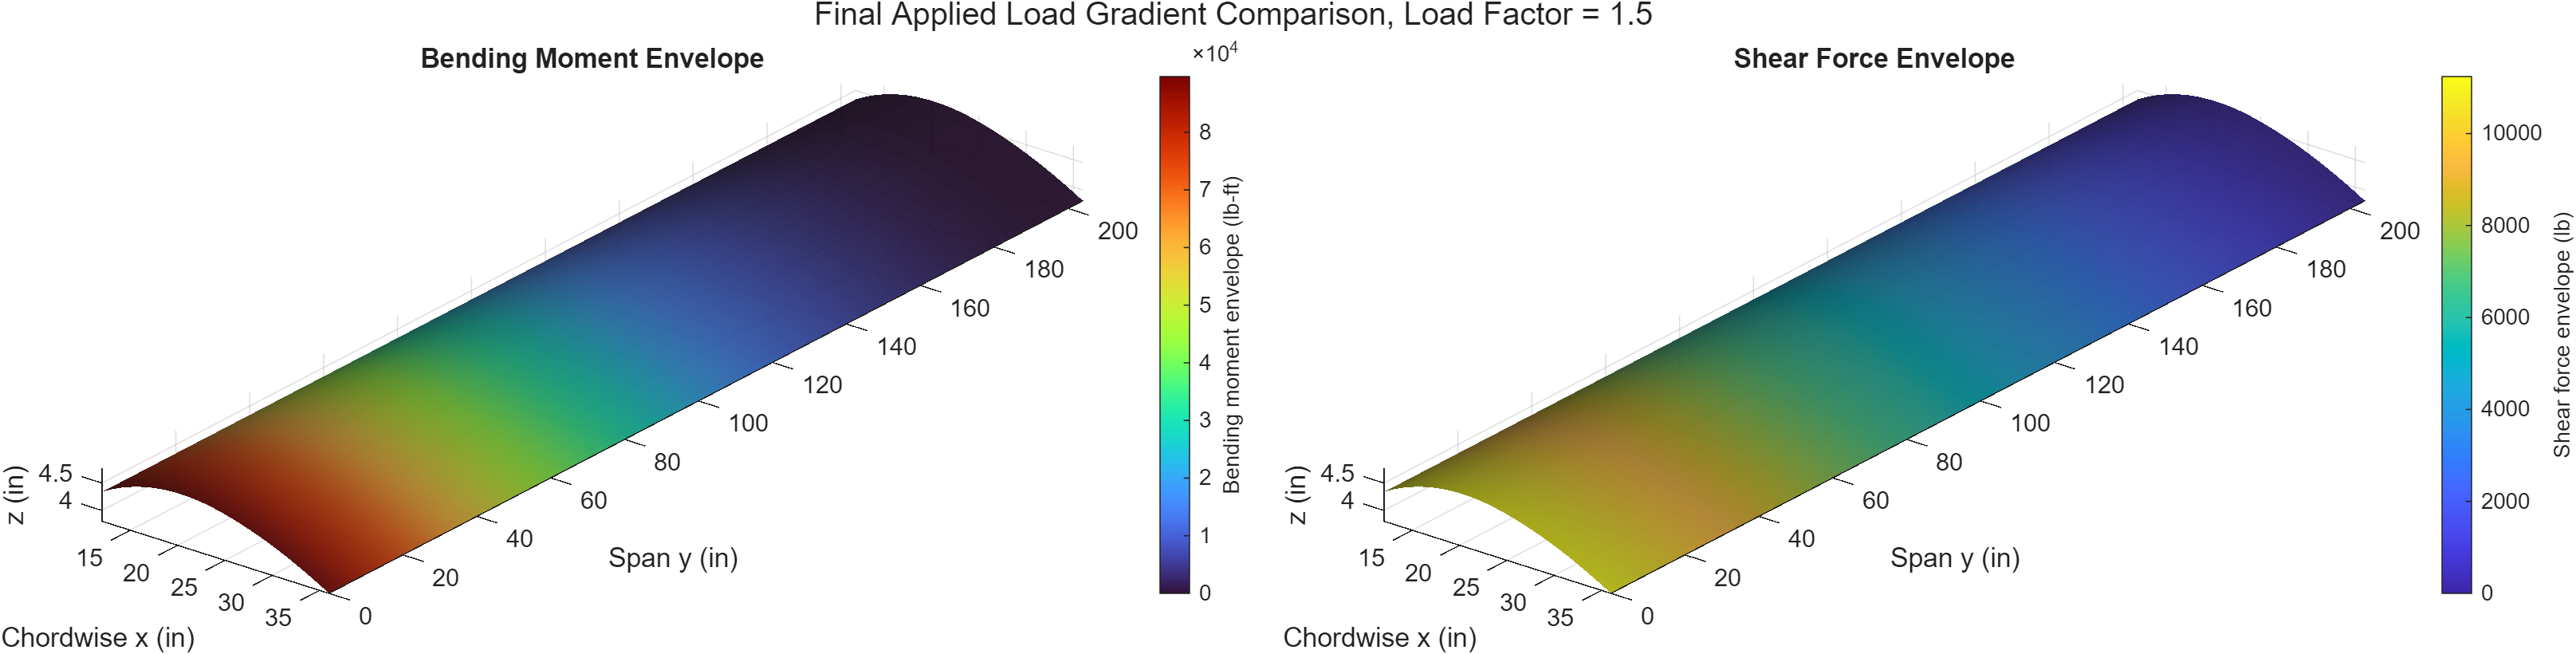
\includegraphics[width=0.95\linewidth]{final_wing_3d_load_gradient_comparison.png}
\caption{Comparison of final bending-moment and shear-force envelopes after ultimate-load scaling. Both gradients are smooth and root-dominated because shear and bending are integrated aerodynamic loads; ribs define structural evaluation stations and do not introduce discontinuities in the applied aerodynamic loads.}
\label{fig:loadgradientcomparison}
\end{figure}

\section{Wing-Box Geometry and Design Variables}

The final wing-box uses a NACA 2412 airfoil, a 60 in chord and a 204 in semispan. The front and rear spars are located at $x/c=0.20$ and $x/c=0.60$, respectively; the rear-spar range used in the final optimisation was constrained to remain at or above $0.60c$ for the final design-space definition. The front and rear spars define the main structural box, while the leading-edge/nose skin ahead of the front spar contributes to the closed thin-walled section and panel idealisation. Figure~\ref{fig:crosssection} shows the final analytical cross section, while Figure~\ref{fig:3dstructure} shows the three-dimensional visualisation of the final wing-box layout.

\begin{figure}[H]
\centering
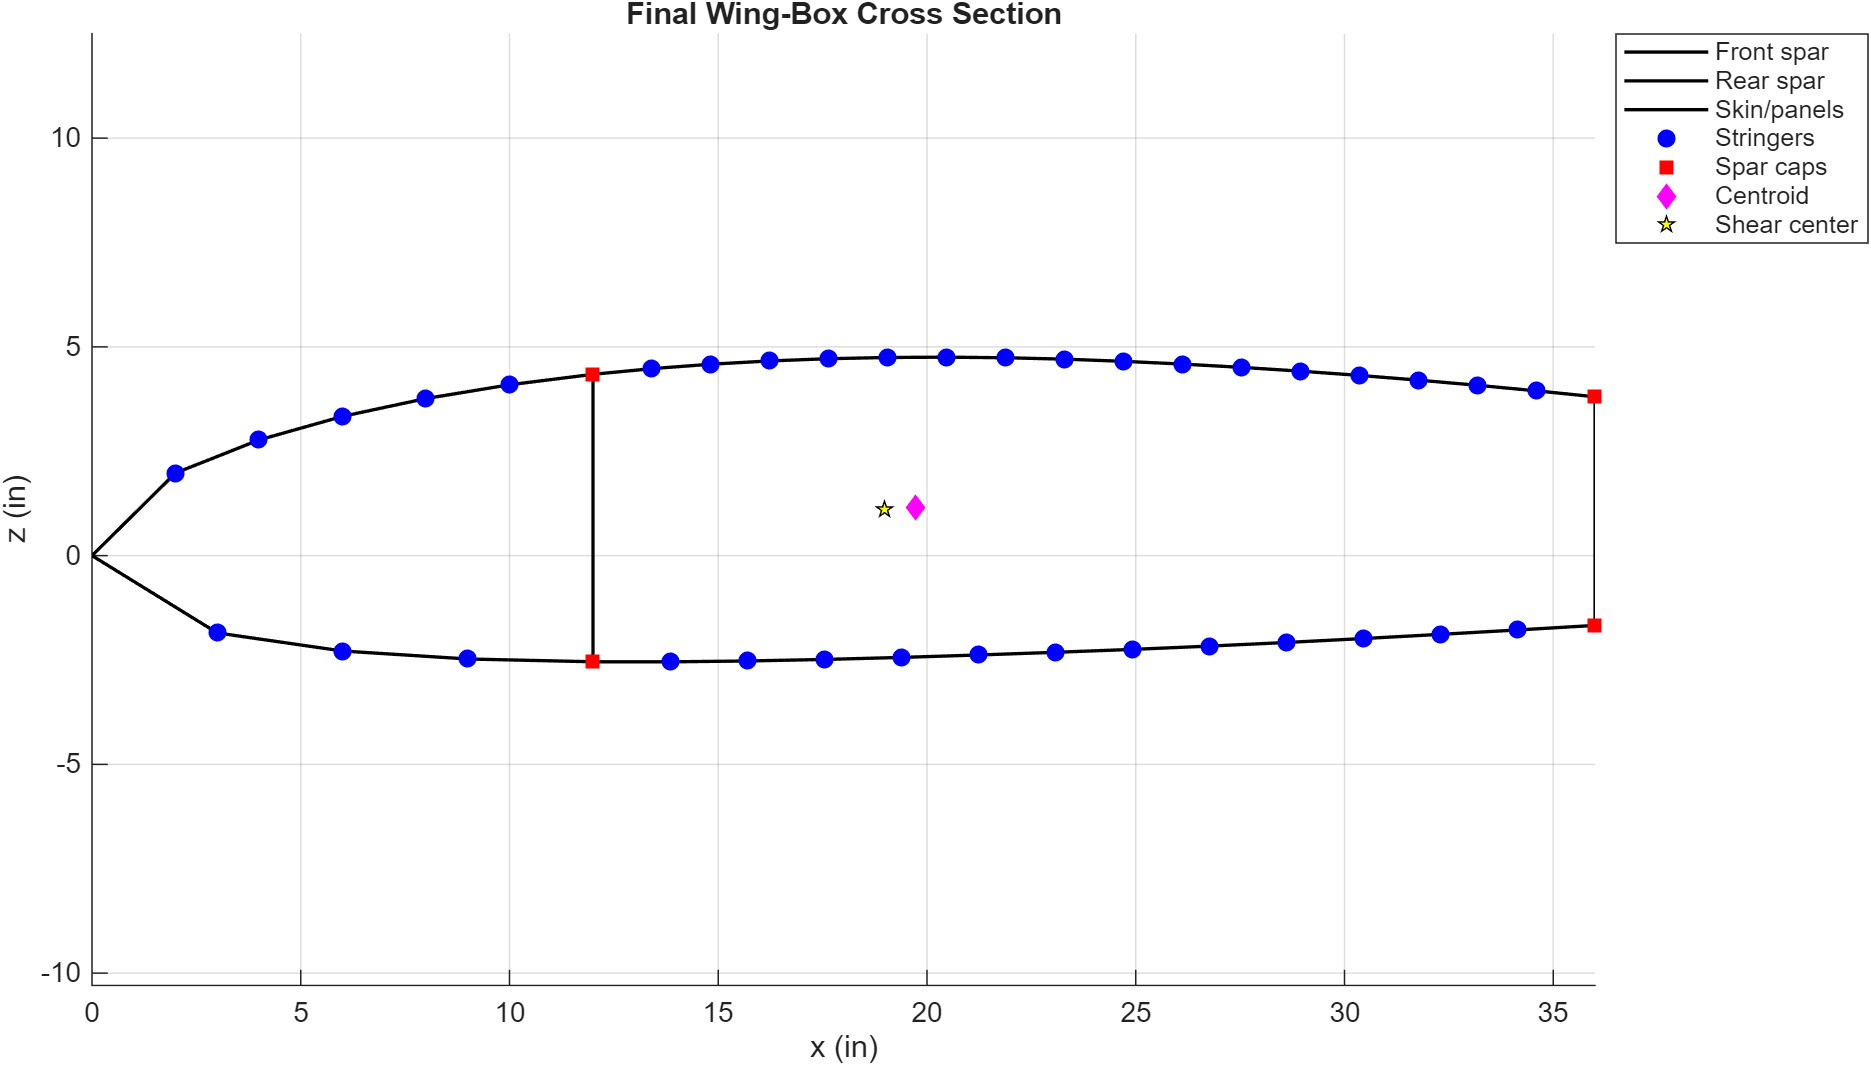
\includegraphics[width=0.80\linewidth]{final_wingbox_cross_section.png}
\caption{Final wing-box cross section with spars, skins, stringers, spar caps, centroid, and shear center.}
\label{fig:crosssection}
\end{figure}

\begin{figure}[H]
\centering
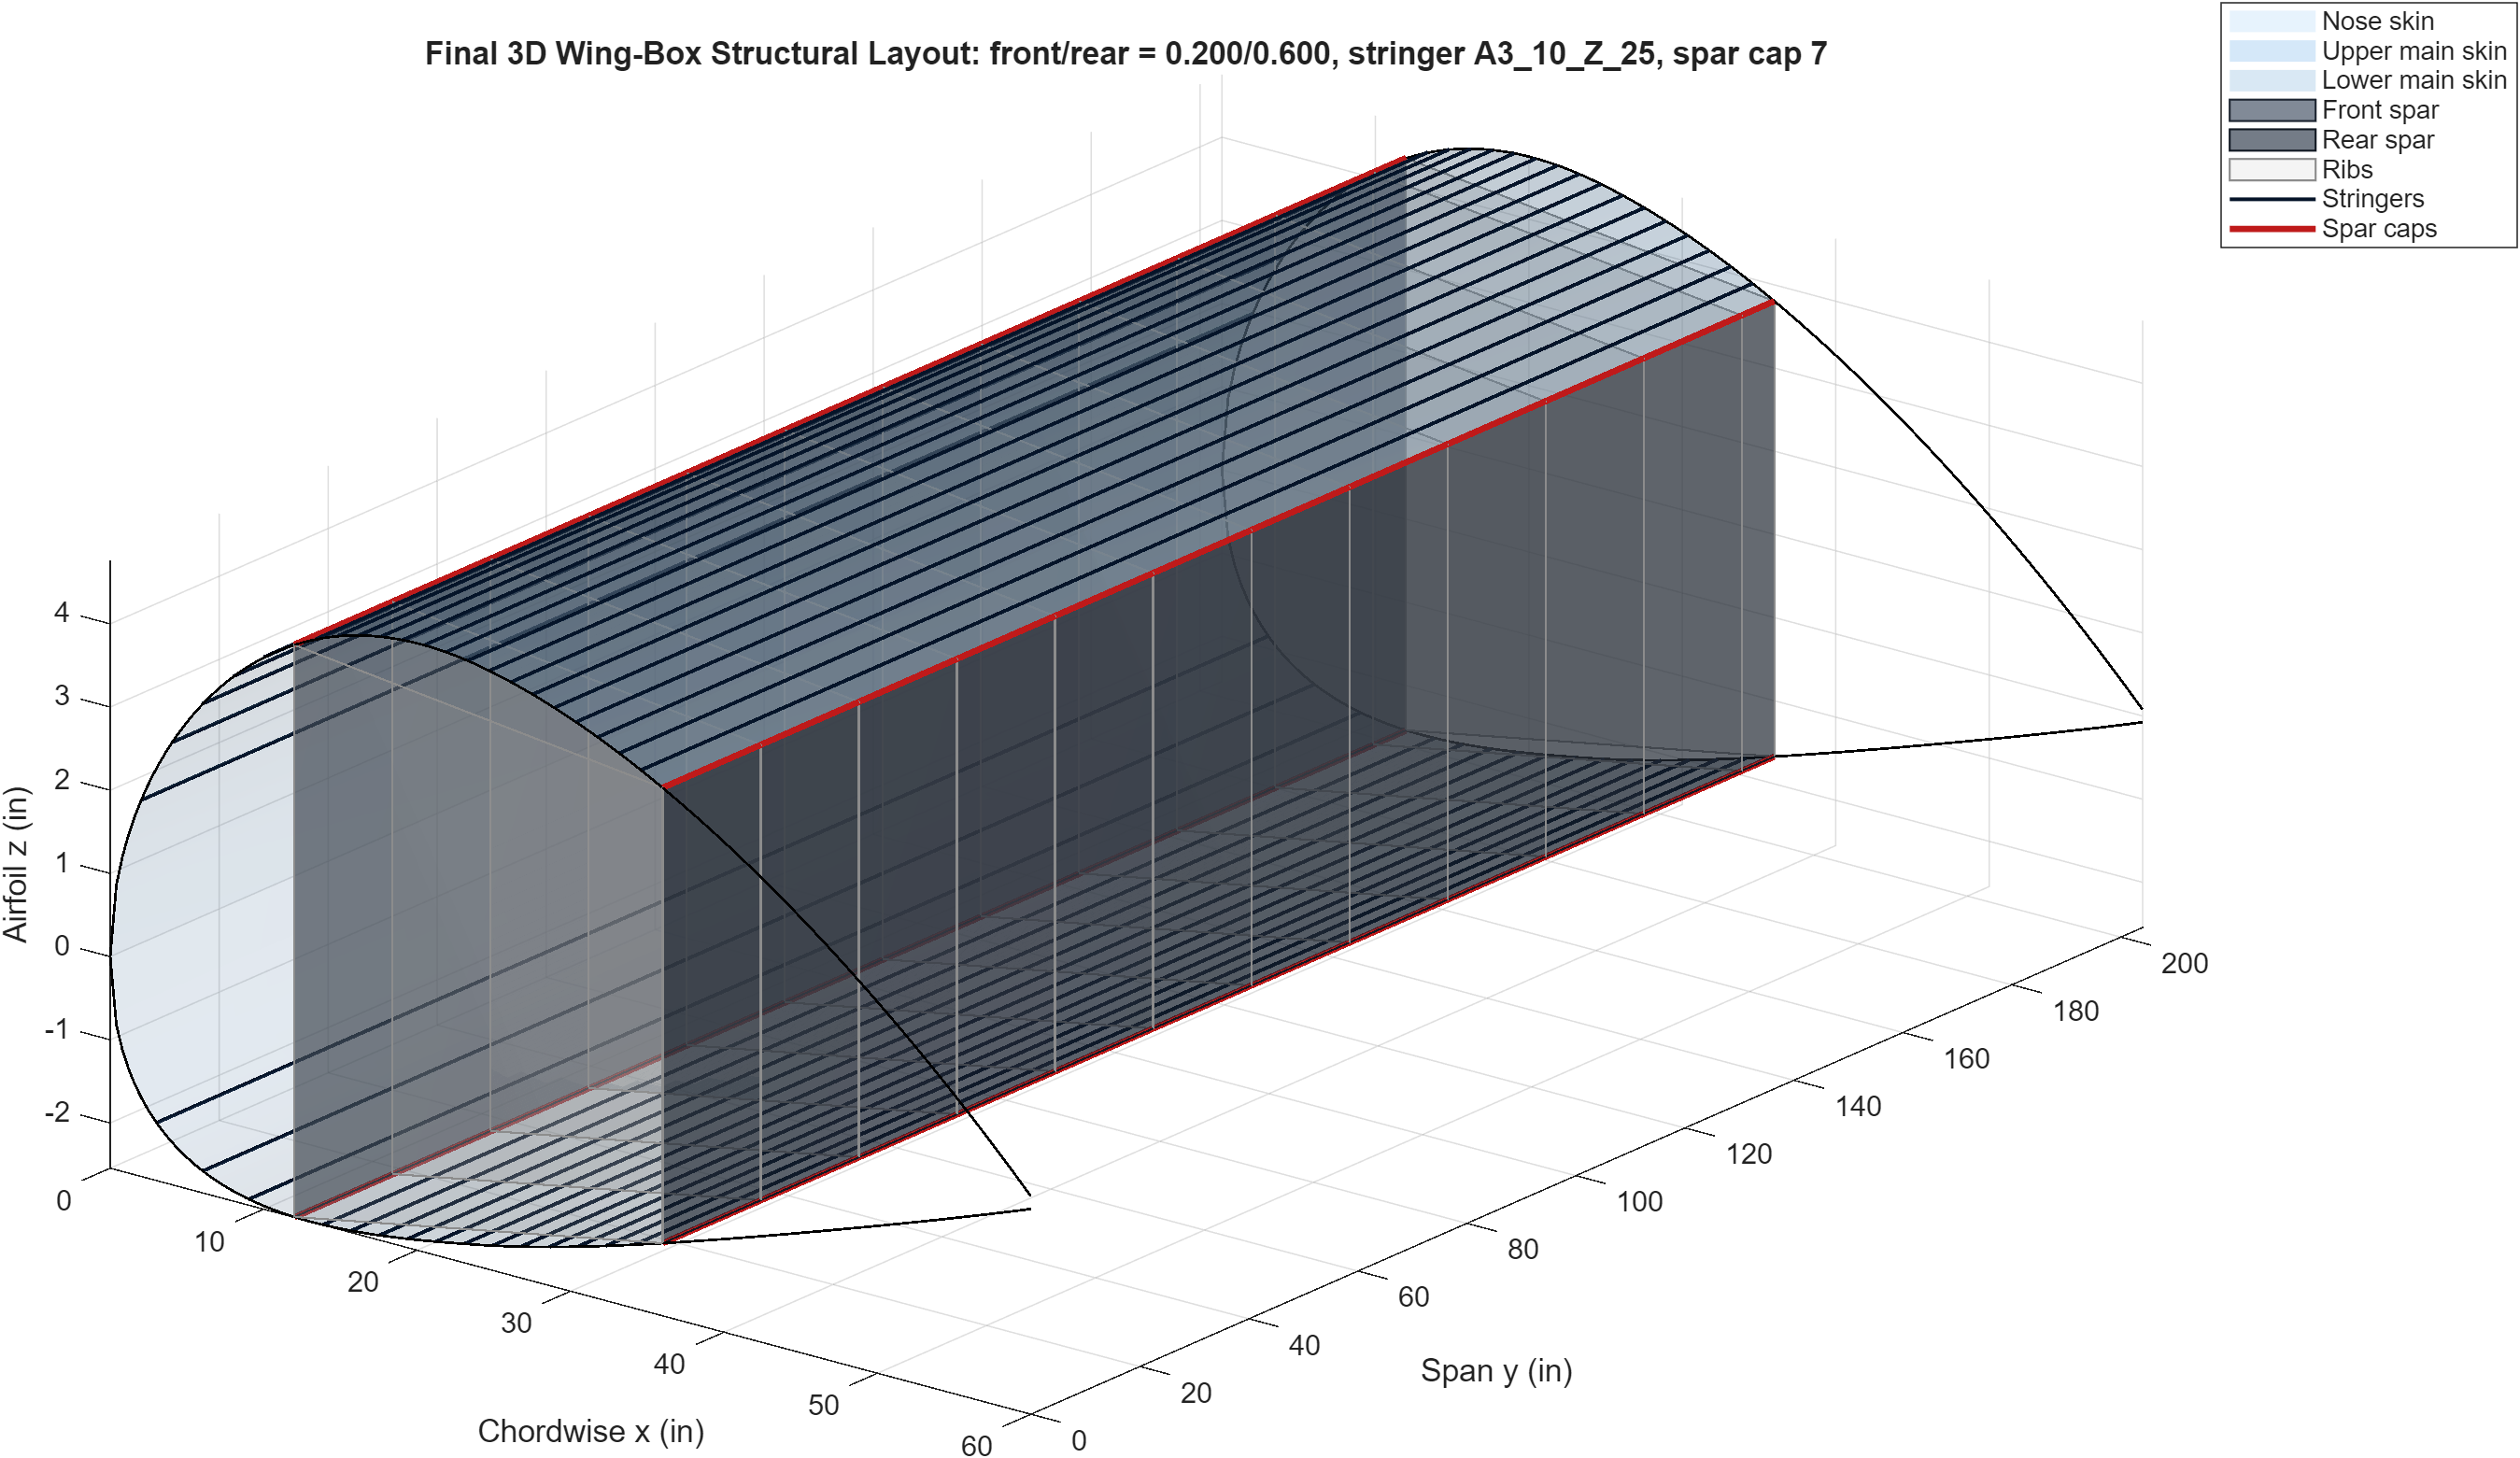
\includegraphics[width=0.95\linewidth]{final_wingbox_3d_structure.png}
\caption{Final three-dimensional wing-box structural visualisation. The transparent nose and main skins show the leading-edge skin, front and rear spar webs, ribs, stringers, and spar caps used by the final structural model.}
\label{fig:3dstructure}
\end{figure}

\begin{table}[H]
\centering
\caption{Final geometry and design variables.}
\label{tab:geometry}
\begin{tabular}{ll}
\toprule
Design variable & Value \\
\midrule
Front / rear spar location & $0.20c$ / $0.60c$ \\
Front / rear spar position & \SI{12}{in} / \SI{36}{in} \\
Main upper/lower skin thickness & \SI{0.056}{in} / \SI{0.056}{in} \\
Nose skin thickness & \SI{0.050}{in} \\
Front / rear spar web thickness & \SI{0.145}{in} / \SI{0.100}{in} \\
Stringer section & A3.10 Z-25 \\
Stringer area & \SI{0.110}{in^2} \\
Spar-cap section & A3.13 T-7 \\
Spar-cap area & \SI{0.240}{in^2} \\
Rib spacing & \SI{18}{in} \\
Fullspan rib count & 25 \\
\bottomrule
\end{tabular}
\end{table}

\section{Materials and Section Selection}

The final material selection uses 2024-T3 sheet for skins, webs, and ribs, with Basis A allowables from MIL-HDBK-5H~\cite{milhdbk5}, and 7075-T6 extrusion properties for stringers and spar caps. The design space uses the extruded Z-sections of Bruhn Table A3.10 for stringers and the T-sections of Bruhn Table A3.13 for spar caps~\cite{bruhn}. These section choices are discrete optimisation variables rather than continuously resized dimensions. The final design uses Bruhn A3.10 Z-section 25 stringers and Bruhn A3.13 T-section 7 spar caps. The Z-stringers provide stiffened-panel axial area and column members along the skins, while the T-section spar caps provide concentrated bending area at the spar lines. This separates sheet-dominated components from extruded stiffening members so that density, elastic constants, and allowables are tied to the intended product form.

\begin{table}[H]
\centering
\caption{Final material groups.}
\label{tab:materials}
\begin{tabular}{lccccc}
\toprule
Component group & Material & $E$ (Msi) & $G$ (Msi) & Density (lb/in$^3$) & Key allowable basis \\
\midrule
Skins, webs, ribs & 2024-T3 sheet & 10.5 & 4.0 & 0.100 & sheet allowables \\
Stringers, spar caps & 7075-T6 extrusion & 10.4 & 3.9 & 0.101 & extrusion allowables \\
\bottomrule
\end{tabular}
\end{table}

\begin{table}[H]
\centering
\caption{Selected stiffener and spar-cap section properties.}
\label{tab:selectedsections}
\scriptsize
\resizebox{\linewidth}{!}{%
\begin{tabular}{>{\raggedright\arraybackslash}p{0.14\linewidth}>{\raggedright\arraybackslash}p{0.14\linewidth}>{\raggedright\arraybackslash}p{0.16\linewidth}>{\raggedright\arraybackslash}p{0.15\linewidth}>{\raggedright\arraybackslash}p{0.10\linewidth}>{\raggedright\arraybackslash}p{0.25\linewidth}}
\toprule
Component & Selected section & Section type & Material group & Area & Key inertia / radius values \\
\midrule
Stringers & A3.10 Z-25 & Bruhn A3.10 Z-section & 7075-T6 extrusion & 0.1100 in$^2$ & $I_{xx}=0.0176$ in$^4$, $I_{yy}=0.0068$ in$^4$; $\rho_{xx}=0.400$ in, $\rho_{yy}=0.249$ in \\
Spar caps & A3.13 T-7 & Bruhn A3.13 T-section & 7075-T6 extrusion & 0.2400 in$^2$ & $\bar{z}=0.327$ in; $I_{yy}=0.0345$ in$^4$, $I_{zz}=0.0188$ in$^4$; $\rho_{xx}=0.379$ in, $\rho_{yy}=0.280$ in \\
\bottomrule
\end{tabular}
}
\end{table}

\section{Structural Analysis Methodology and Equations}

\subsection{Unit-Load Response Formulation}

The structural solver separates geometry-dependent section response from case-dependent load magnitudes. For each candidate geometry, the section analysis first computes the unit bending-stress coefficients and unit shear-flow coefficients associated with the structural load components. The load-interpolation step provides ultimate-load values of $V_x$, $V_z$, $M_x$, $M_z$, and $M_y$ at each rib station. These values already include the 1.5 load factor before they enter the unit-response superposition, so the stress and shear-flow recovery equations use them directly.

\begin{equation}
  \sigma(y,\mathrm{case}) =
  M_x(y,\mathrm{case})\,\sigma_{M_x}^{unit}
  +
  M_z(y,\mathrm{case})\,\sigma_{M_z}^{unit}
\end{equation}

\begin{equation}
  q(y,\mathrm{case}) =
  V_x(y,\mathrm{case})\,q_{V_x}^{unit}
  +
  V_z(y,\mathrm{case})\,q_{V_z}^{unit}
  +
  M_y(y,\mathrm{case})\,q_{M_y}^{unit}
\end{equation}

\begin{equation}
  \tau(y,\mathrm{case}) = \frac{q(y,\mathrm{case})}{t}
\end{equation}

The $V_z$ unit shear-flow term includes the moment arm between the shear center and the aerodynamic quarter-chord reference, so the model includes vertical-load torsion through the shear-flow coefficient rather than modifying the aerodynamic pitching-moment input. This formulation lets the solver evaluate all nine load cases consistently for each candidate geometry because it computes the geometry-dependent coefficients once and then reuses them with the interpolated loads.

\subsection{Section Idealisation and Bending Stress}

The final section model uses a modified form of the Megson panel idealisation~\cite{megson} to distribute effective panel axial area to adjacent booms based on the section $z$-ratio method. For a thin panel between boom endpoints, the equivalent boom-area contribution follows the Megson concept of matching the direct-stress resultant from a linearly varying panel stress distribution. This gives the skins and spar webs axial stiffness in the idealised section without counting the physical panel material twice in the weight model. The panel idealisation affects centroid location, inertias, bending stresses, shear-flow coefficients, shear center, and downstream checks. Physical panel weight is still computed from the actual panel geometry and thicknesses.

Bending stresses are recovered from the section properties and applied bending moments. In simplified notation, neglecting coupling terms, the direct stress contribution may be written as
\begin{equation}
  \sigma = -\frac{M_x z}{I_{xx}} + \frac{M_z x}{I_{zz}},
\end{equation}
with the implemented section analysis using the sign convention of the model and the computed section inertias, including the nonzero product-of-inertia contribution where present.

\subsection{Shear Flow and Torsion}

The shear-flow calculation combines shear and torsional contributions,
\begin{equation}
  q = q_{\mathrm{shear}} + q_{\mathrm{torsion}}.
\end{equation}
The implementation evaluates this expression through unit shear-flow coefficients for $V_x$, $V_z$, and $M_y$. The $V_z$ unit shear-flow coefficient includes the moment arm between the shear center and the aerodynamic quarter-chord reference, so the model includes shear-center torsion from vertical load without modifying the aerodynamic $M_y$ data.

\subsection{Yield and Von Mises Screening}

The yield screen computes panel von Mises stress with the plane-stress form
\begin{equation}
  \sigma_{\mathrm{vm}} = \sqrt{\sigma^2 + 3\tau^2}.
\end{equation}
The yield ratio is
\begin{equation}
  R_y = \frac{\sigma_{\mathrm{vm}}}{\sigma_y}.
\end{equation}
The model uses panel stresses recovered from the adjacent idealised section elements and then evaluates panel and bay checks using the physical panel geometry.

\subsection{Euler Column Buckling}

Discrete compression-member Euler buckling is checked using
\begin{equation}
  P_{\mathrm{cr}} = \frac{\pi^2 E I}{(K L)^2},
\end{equation}
with $K_{\mathrm{column}} = 0.7$. The effective column length is tied to the rib spacing.
The column check applies to discrete compression members such as stringers and spar caps. It is separate from local crippling; crippling is outside the numerical scope of this report.

\subsection{Panel Buckling and Combined Ratios}

Panel buckling uses separate compression, bending, and shear ratios,
\begin{equation}
  R_c = \frac{\sigma_c}{\sigma_{c,\mathrm{cr}}}, \qquad
  R_b = \frac{\sigma_b}{\sigma_{b,\mathrm{cr}}}, \qquad
  R_s = \frac{\tau}{\tau_{\mathrm{cr}}},
\end{equation}
with fixed coefficients $K_c=6$, $K_b=32$, and $K_s=8$. The corresponding flat-panel critical stresses use
\begin{equation}
  \sigma_{c,\mathrm{cr}} =
  \frac{K_c \pi^2 E_c}{12(1-\nu^2)}\left(\frac{t}{b}\right)^2,
  \qquad
  \sigma_{b,\mathrm{cr}} =
  \frac{K_b \pi^2 E_c}{12(1-\nu^2)}\left(\frac{t}{b}\right)^2,
\end{equation}
\begin{equation}
  \tau_{\mathrm{cr}} =
  \frac{K_s \pi^2 E}{12(1-\nu^2)}\left(\frac{t}{b}\right)^2.
\end{equation}
The final panel buckling recovery uses bay-averaged stresses and shear flow: the method recovers compression from the four surrounding boom/stringer stresses for the panel bay and averages shear between adjacent rib stations. The compression critical stress includes the curved-panel correction where applicable; spar webs remain flat-panel checks, and bending and shear buckling remain flat-panel checks.

The panel buckling check evaluates the combined ratios as
\begin{equation}
  R_{SC} = R_s^{1.5} + R_c,
\end{equation}
for shear plus compression and
\begin{equation}
  R_{BS} = R_b^2 + R_s^2,
\end{equation}
for bending plus shear.

\subsection{Divergence}

Divergence is expressed as the ratio between the computed divergence speed and the dive speed $V_D=\SI{270}{mph}$,
\begin{equation}
  R_{\mathrm{div}} = \frac{V_{\mathrm{div}}}{V_D}.
\end{equation}
A divergence ratio greater than 1 indicates pass for the implemented check.

\subsection{Rib Weight Model}

The geometric rib weight model is
\begin{equation}
  W_{\mathrm{rib}} = \rho t f_{\mathrm{solid}} A_{\mathrm{NACA}},
\end{equation}
where $A/c^2=0.082169$, $c=\SI{60}{in}$, $f_{\mathrm{solid}}=0.7$, and rib thickness is \SI{0.040}{in}. The resulting single-rib weight is approximately \SI{0.8283}{lb}.

\section{Adaptive Monte Carlo Optimisation}

The final optimisation followed an intentional two-level engineering workflow. First, manual verification sweeps were used to confirm that the structural model responded sensibly to key variables such as spar web thickness, nose skin thickness, main skin thickness, rib spacing, and panel buckling utilisation. These sweeps established feasible design regions and confirmed that the primary constraints were yield, local panel buckling, and combined panel loading rather than divergence.

The final optimisation then used a four-stage adaptive Monte Carlo search. Each stage evaluated 5000 random designs, for 20,000 total designs. Of these, 2596 passed all implemented checks. Ranges were refined using elite passing designs after each stage; the retained elite set was the best 10 percent of passing designs, subject to a minimum elite count. The refined variables were
\[
\begin{gathered}
  x_{f}/c,\; x_{r}/c,\; t_{\mathrm{main}},\; t_{\mathrm{nose}},\;
  t_{\mathrm{front\,web}},\; t_{\mathrm{rear\,web}},\\
  N_{\mathrm{top}},\; N_{\mathrm{bottom}},\; N_{\mathrm{nose,top}},\;
  N_{\mathrm{nose,bottom}},\; s_{\mathrm{rib}},\;
  \mathrm{stringer\ section},\; \mathrm{spar\ cap\ section}.
\end{gathered}
\]
The selected design comes from Stage 2, since it is the lightest passing candidate found across all four stages. The Stage 4 best still supports the convergence discussion, but it is not the selected final candidate.

\begin{table}[H]
\centering
\caption{Adaptive Monte Carlo stage summary.}
\label{tab:mcstage}
\begin{tabular}{ccccc}
\toprule
Stage & Designs & Passing & Pass rate & Best weight (lb) \\
\midrule
1 & 5000 & 876 & 17.52\% & 471.5754 \\
2 & 5000 & 620 & 12.40\% & 449.4477 \\
3 & 5000 & 569 & 11.38\% & 460.1662 \\
4 & 5000 & 531 & 10.62\% & 458.7316 \\
\bottomrule
\end{tabular}
\end{table}

\begin{figure}[H]
\centering
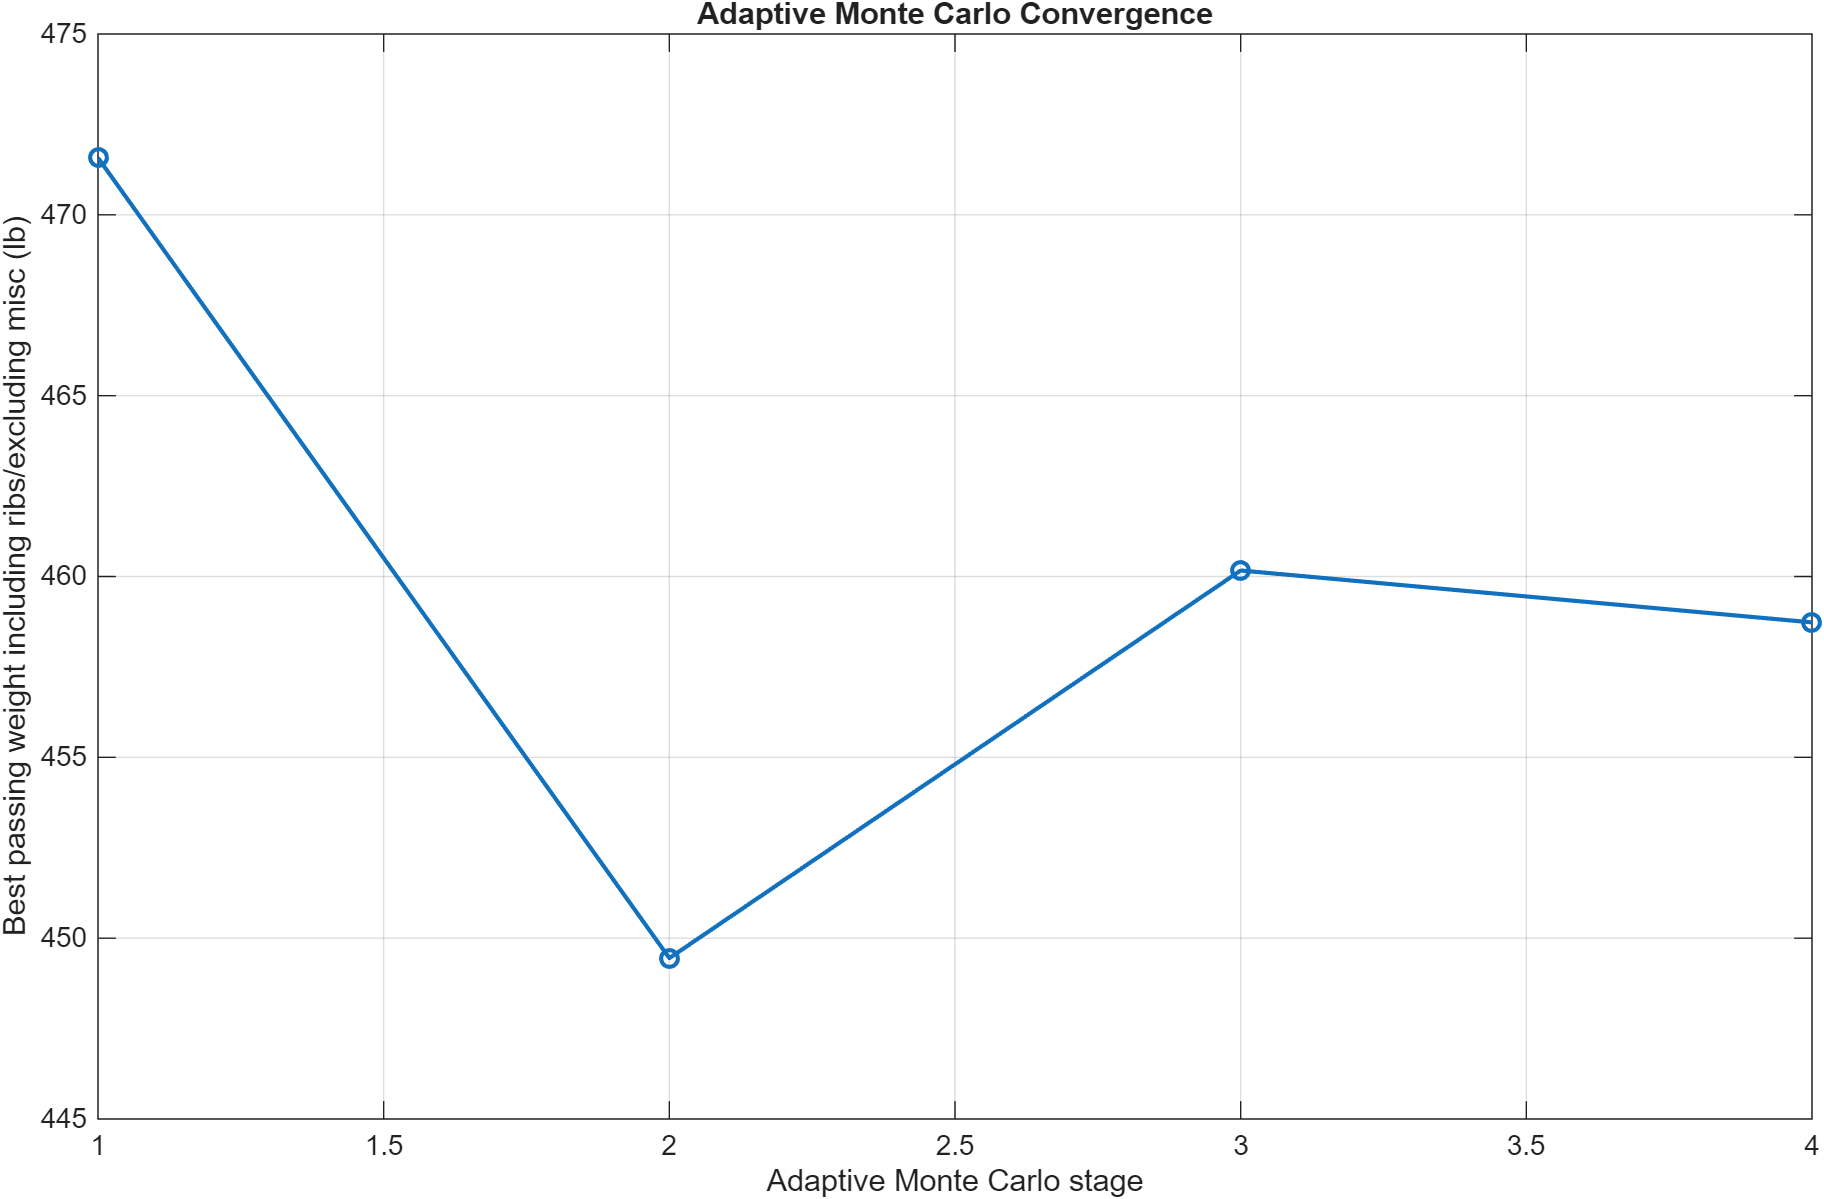
\includegraphics[width=0.82\linewidth]{final_adaptive_convergence.png}
\caption{Best passing weight by adaptive Monte Carlo stage. Stage 2 contains the global best.}
\label{fig:mcconvergence}
\end{figure}

\begin{figure}[H]
\centering
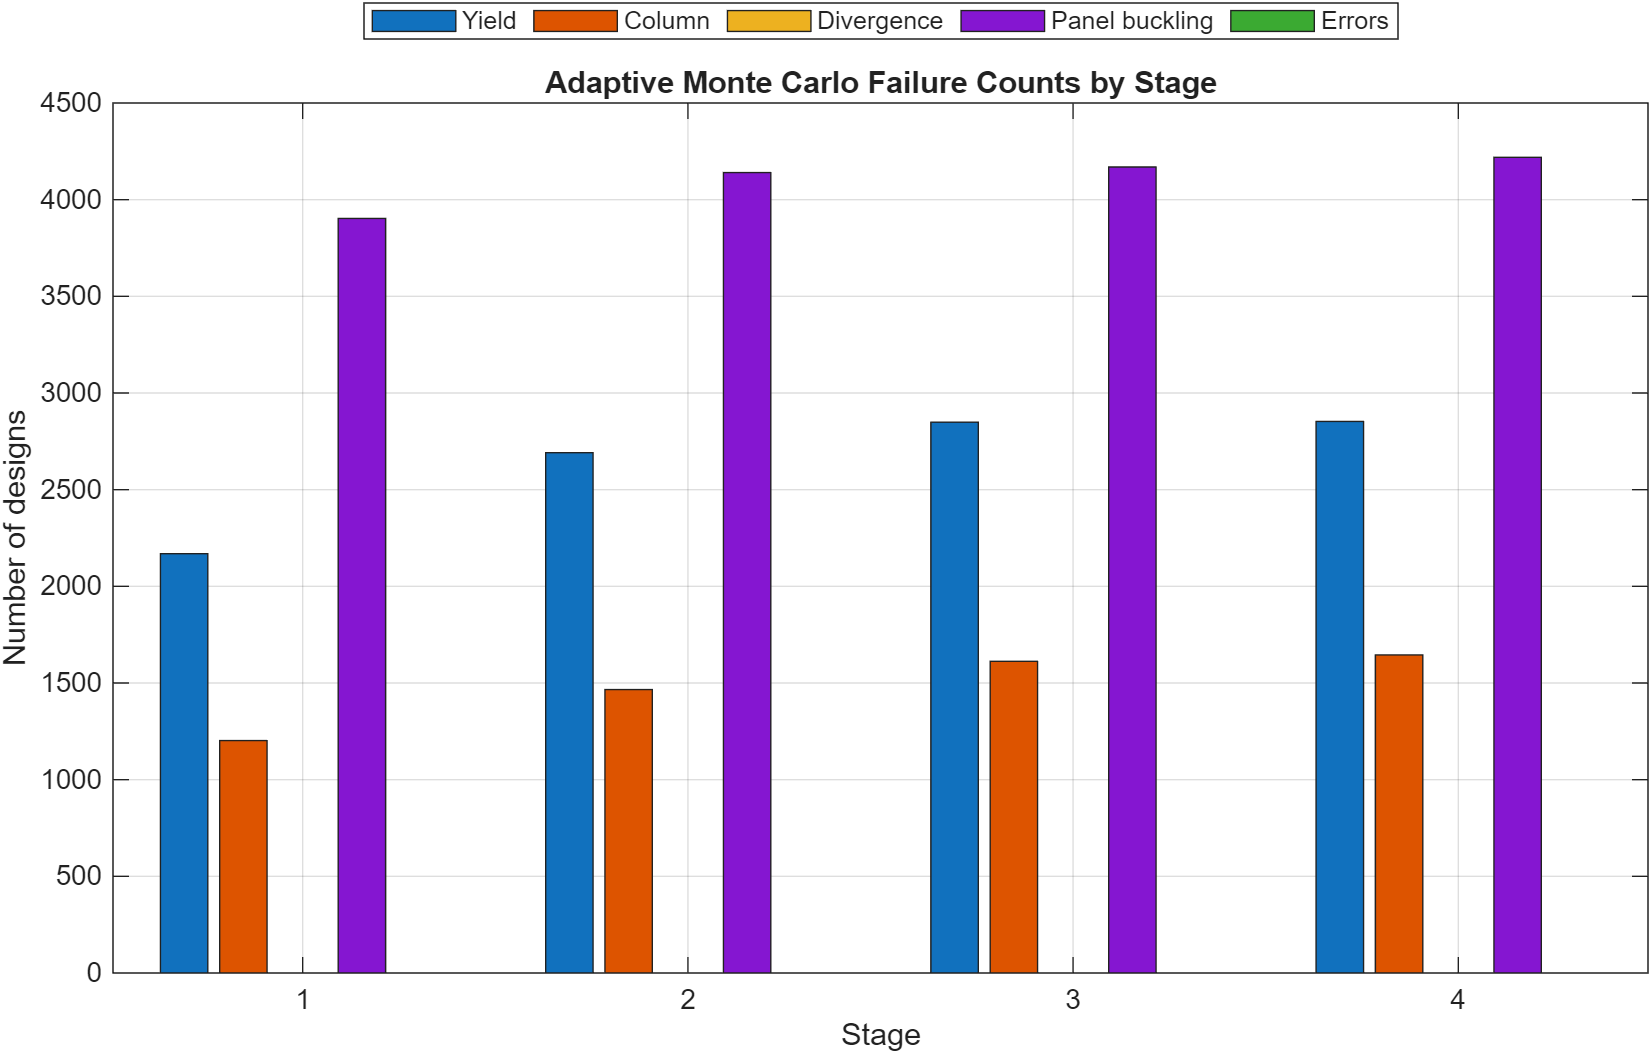
\includegraphics[width=0.82\linewidth]{final_adaptive_failure_breakdown_by_stage.png}
\caption{Failure counts by stage for the implemented checks. Failure categories are not mutually exclusive because one sampled design can fail multiple checks.}
\label{fig:mcfailure}
\end{figure}

\begin{table}[H]
\centering
\caption{Adaptive Monte Carlo failure breakdown by stage.}
\label{tab:mcfailure}
\begin{tabular}{cccccc}
\toprule
Stage & Yield & Column & Divergence & Panel buckling & Errors \\
\midrule
1 & 2169 & 1202 & 0 & 3903 & 0 \\
2 & 2691 & 1466 & 0 & 4140 & 0 \\
3 & 2849 & 1612 & 0 & 4169 & 0 \\
4 & 2853 & 1645 & 0 & 4219 & 0 \\
\bottomrule
\end{tabular}
\end{table}

\begin{figure}[H]
\centering
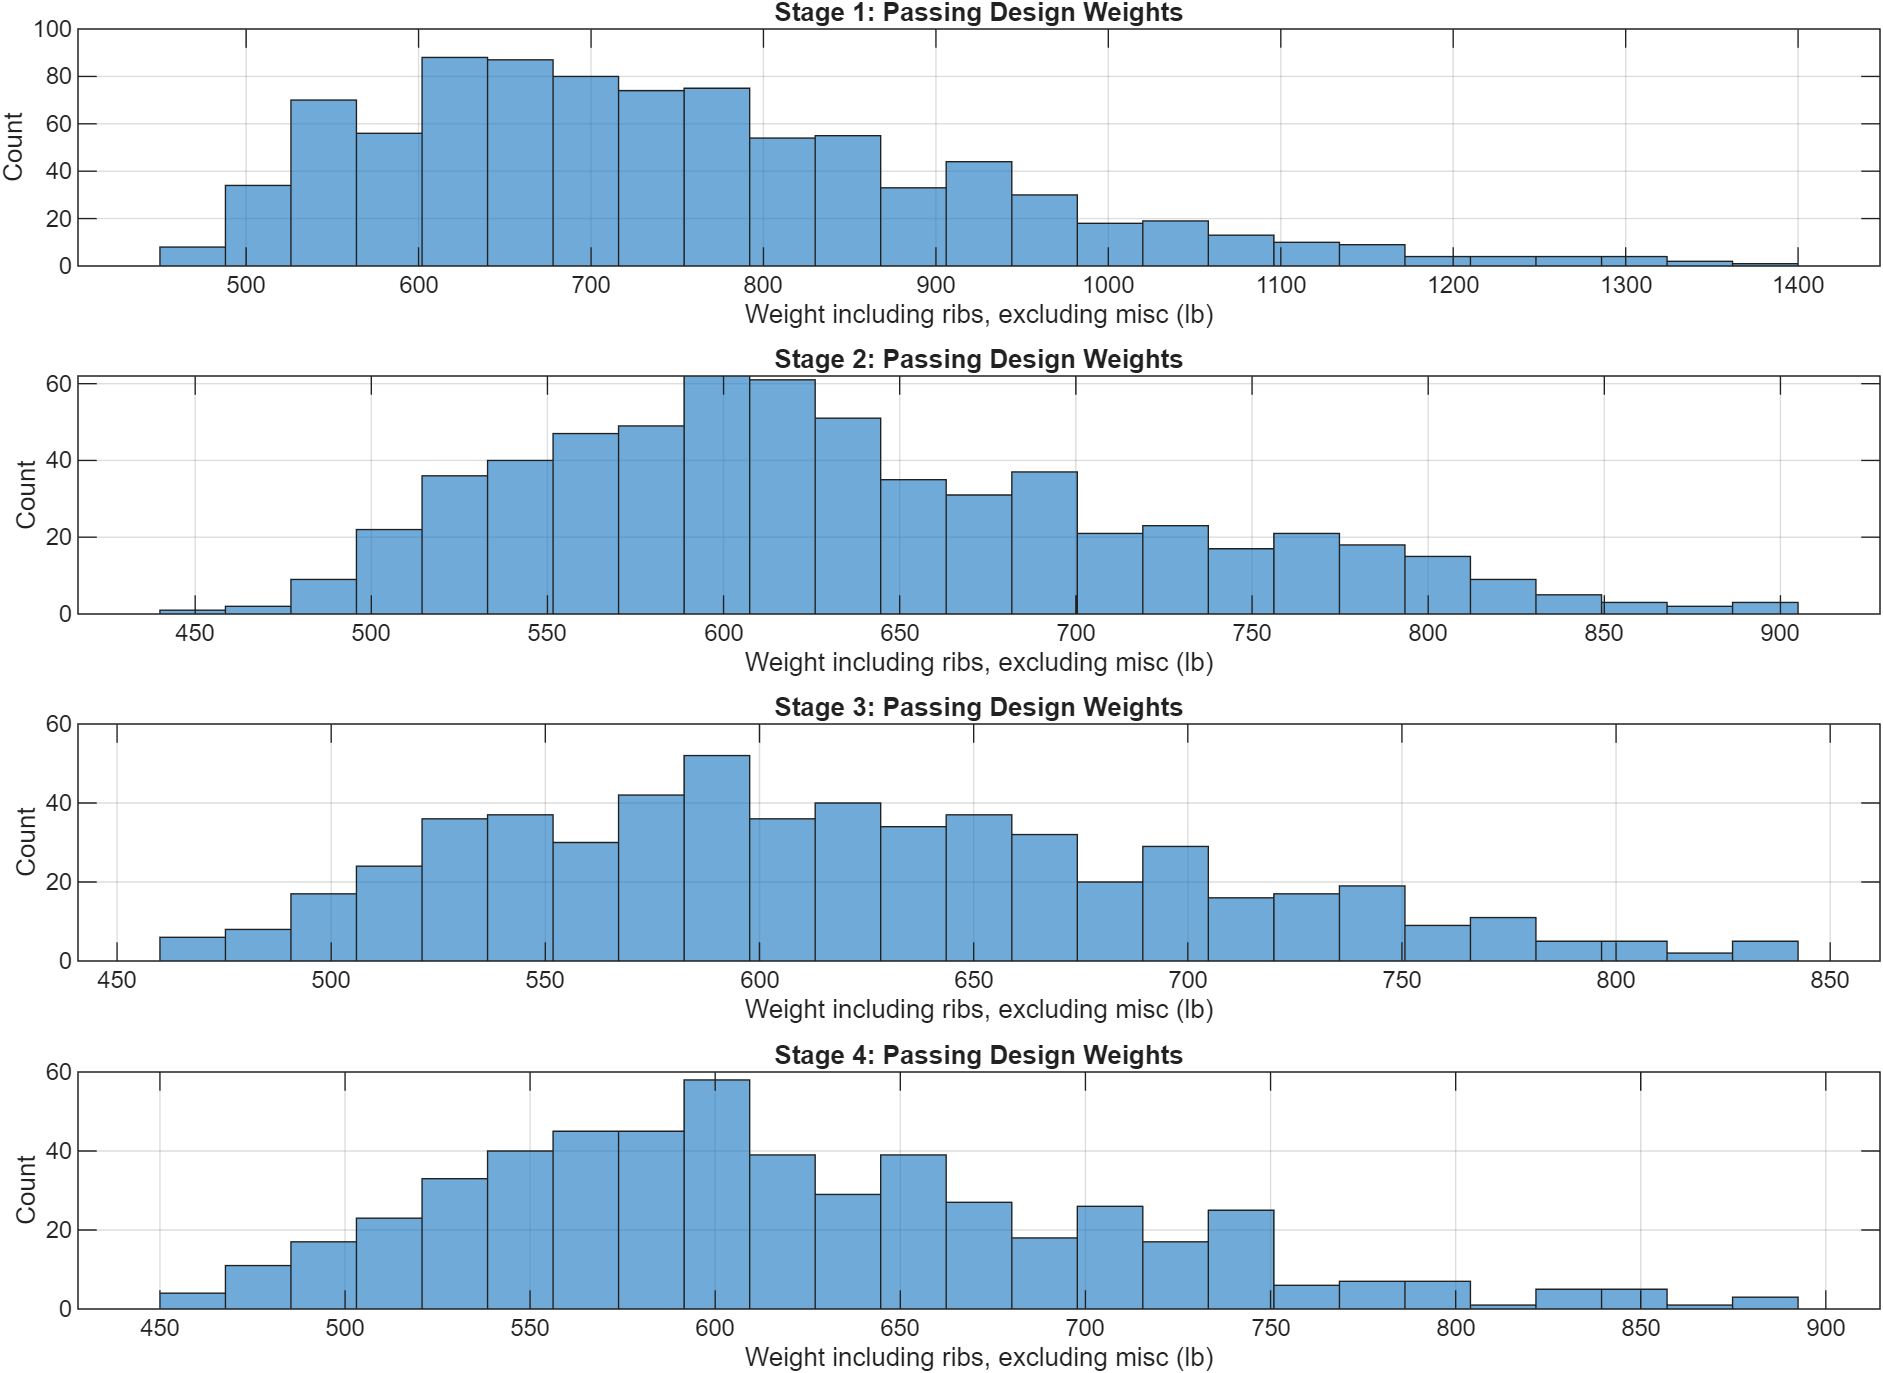
\includegraphics[width=0.88\linewidth]{final_adaptive_passing_weight_histogram_by_stage.png}
\caption{Passing-design weight distributions by adaptive stage. The histograms show how the adaptive search concentrated around lower-weight feasible candidates while still retaining a spread of passing designs.}
\label{fig:passinghist}
\end{figure}

\begin{figure}[H]
\centering
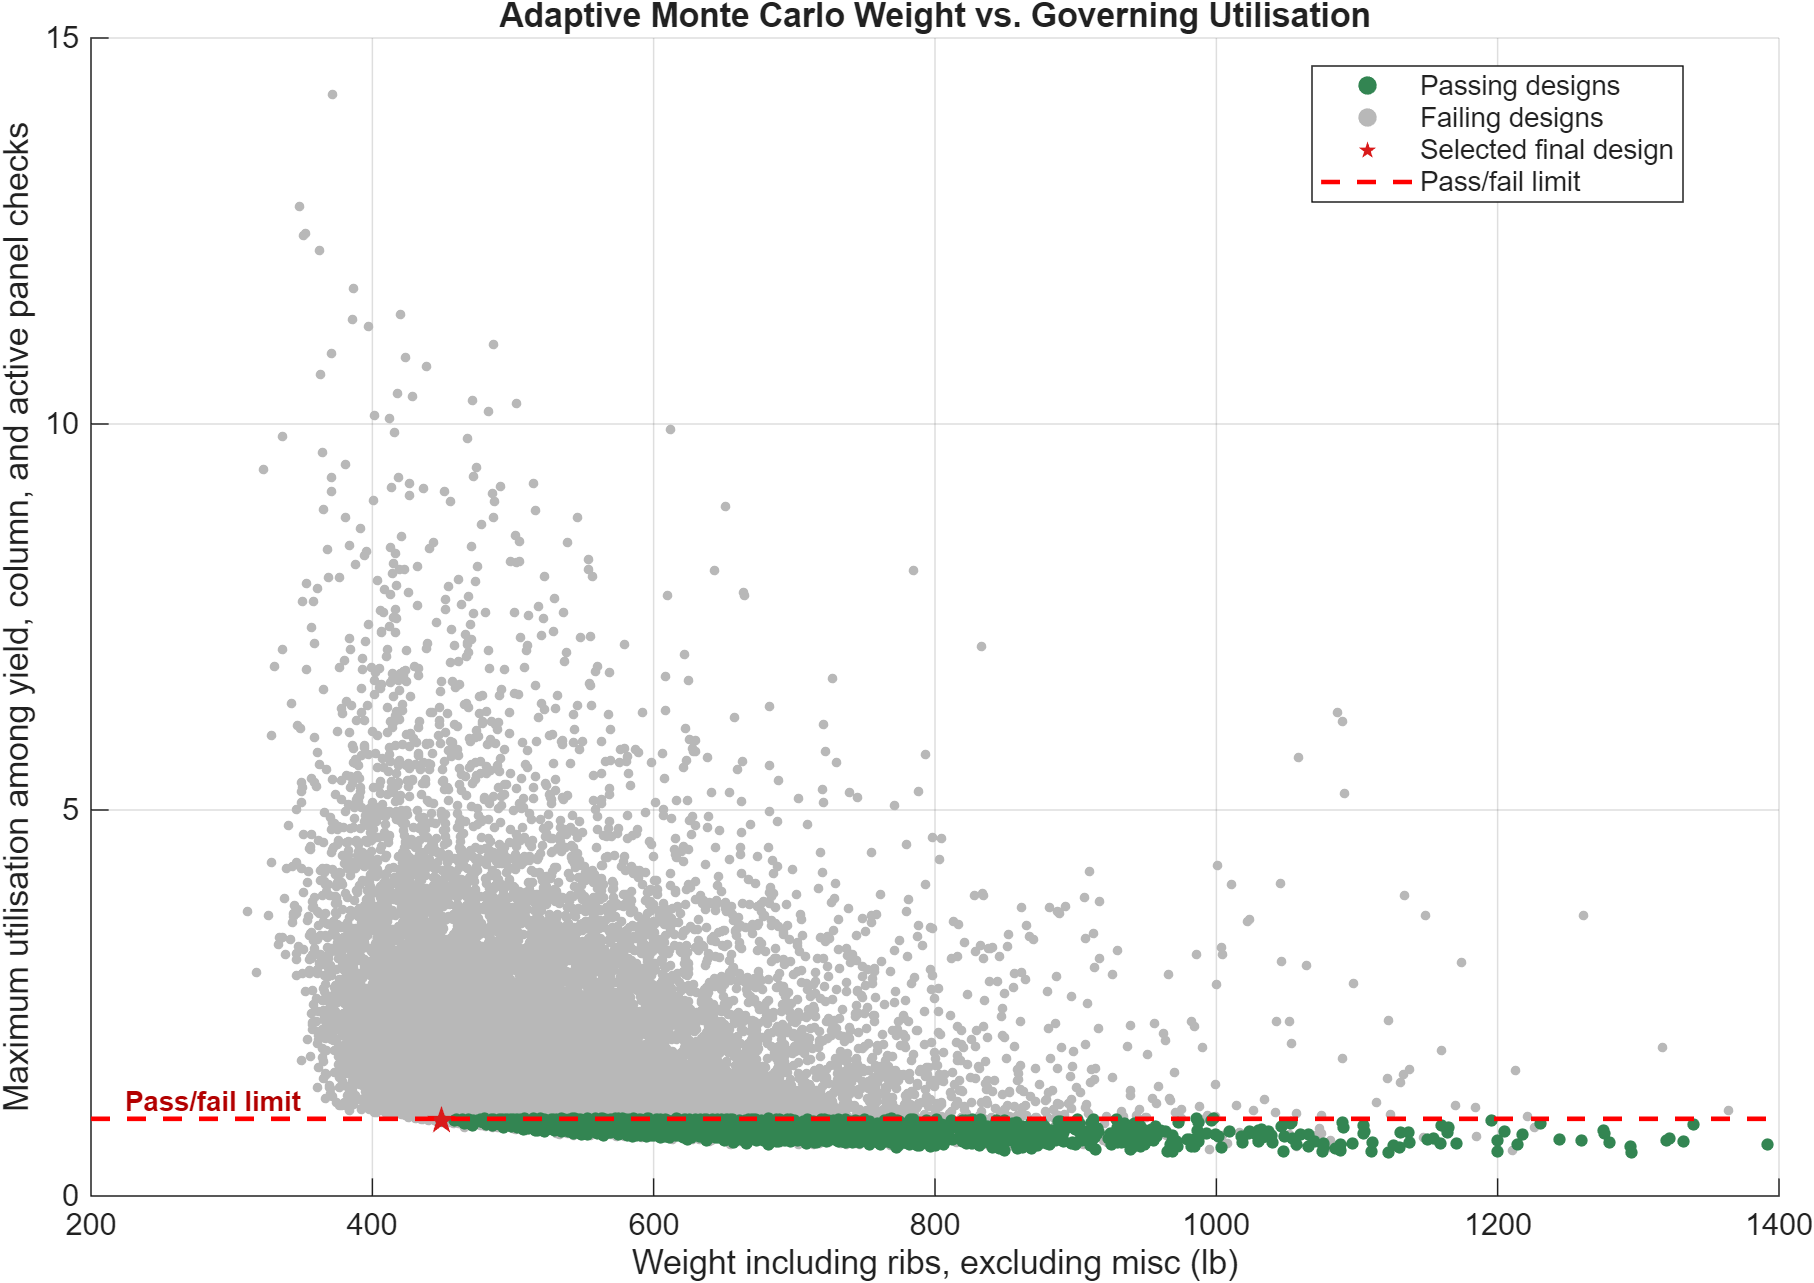
\includegraphics[width=0.82\linewidth]{final_adaptive_weight_vs_utilisation.png}
\caption{Adaptive Monte Carlo weight versus governing utilisation.}
\label{fig:weightutil}
\end{figure}

The adaptive Monte Carlo result is not a proof of a deterministic global mathematical optimum. It is the lightest passing design found by the final adaptive random search under the specified design-variable ranges and implemented analysis checks.

\section{Final Optimised Design}

Table~\ref{tab:finaldesign} gives the final weight and status summary for the design defined in Table~\ref{tab:geometry}. The selected candidate is the global best across all adaptive stages and passes all implemented structural checks.

\begin{table}[H]
\centering
\caption{Final optimised design result summary.}
\label{tab:finaldesign}
\begin{tabular}{ll}
\toprule
Quantity & Value \\
\midrule
Weight including ribs, excluding misc. & \SI{449.4477}{lb} \\
Weight excluding ribs and misc. & \SI{428.7410}{lb} \\
Rib weight, fullspan & \SI{20.7067}{lb} \\
Overall implemented-check status & Pass \\
\bottomrule
\end{tabular}
\end{table}

\section{Structural Response and Failure Assessment}

The final structural response is summarised in Table~\ref{tab:failures}. All implemented checks pass. The active combined panel buckling ratio is well below 1, while yield is the tightest final screening margin.

Figure~\ref{fig:utilbars} plots the major checks on a common utilisation scale. Yield, column buckling, and active panel combined ratios are already ratios to their pass/fail limits. Divergence is plotted as $1/R_{\mathrm{div}}$ so that all bars share a common limit of 1.0.

\begin{table}[H]
\centering
\caption{Final implemented failure-check summary.}
\label{tab:failures}
\begin{tabular}{lcc}
\toprule
Check & Ratio/value & Status \\
\midrule
Yield ratio & 0.9744 & Pass \\
Euler column buckling ratio & 0.8643 & Pass \\
Divergence ratio & 4.8712 & Pass \\
Panel compression ratio, $R_c$ & 0.9167 & Pass \\
Panel bending ratio, $R_b$ & 0.1929 & Pass \\
Panel shear ratio, $R_s$ & 0.3393 & Pass \\
Active combined panel ratio & 0.3372 & Pass \\
\bottomrule
\end{tabular}
\end{table}

The controlling active combined panel ratio occurs near the root under the PHAA load case, in shear-plus-compression.

\begin{figure}[H]
\centering
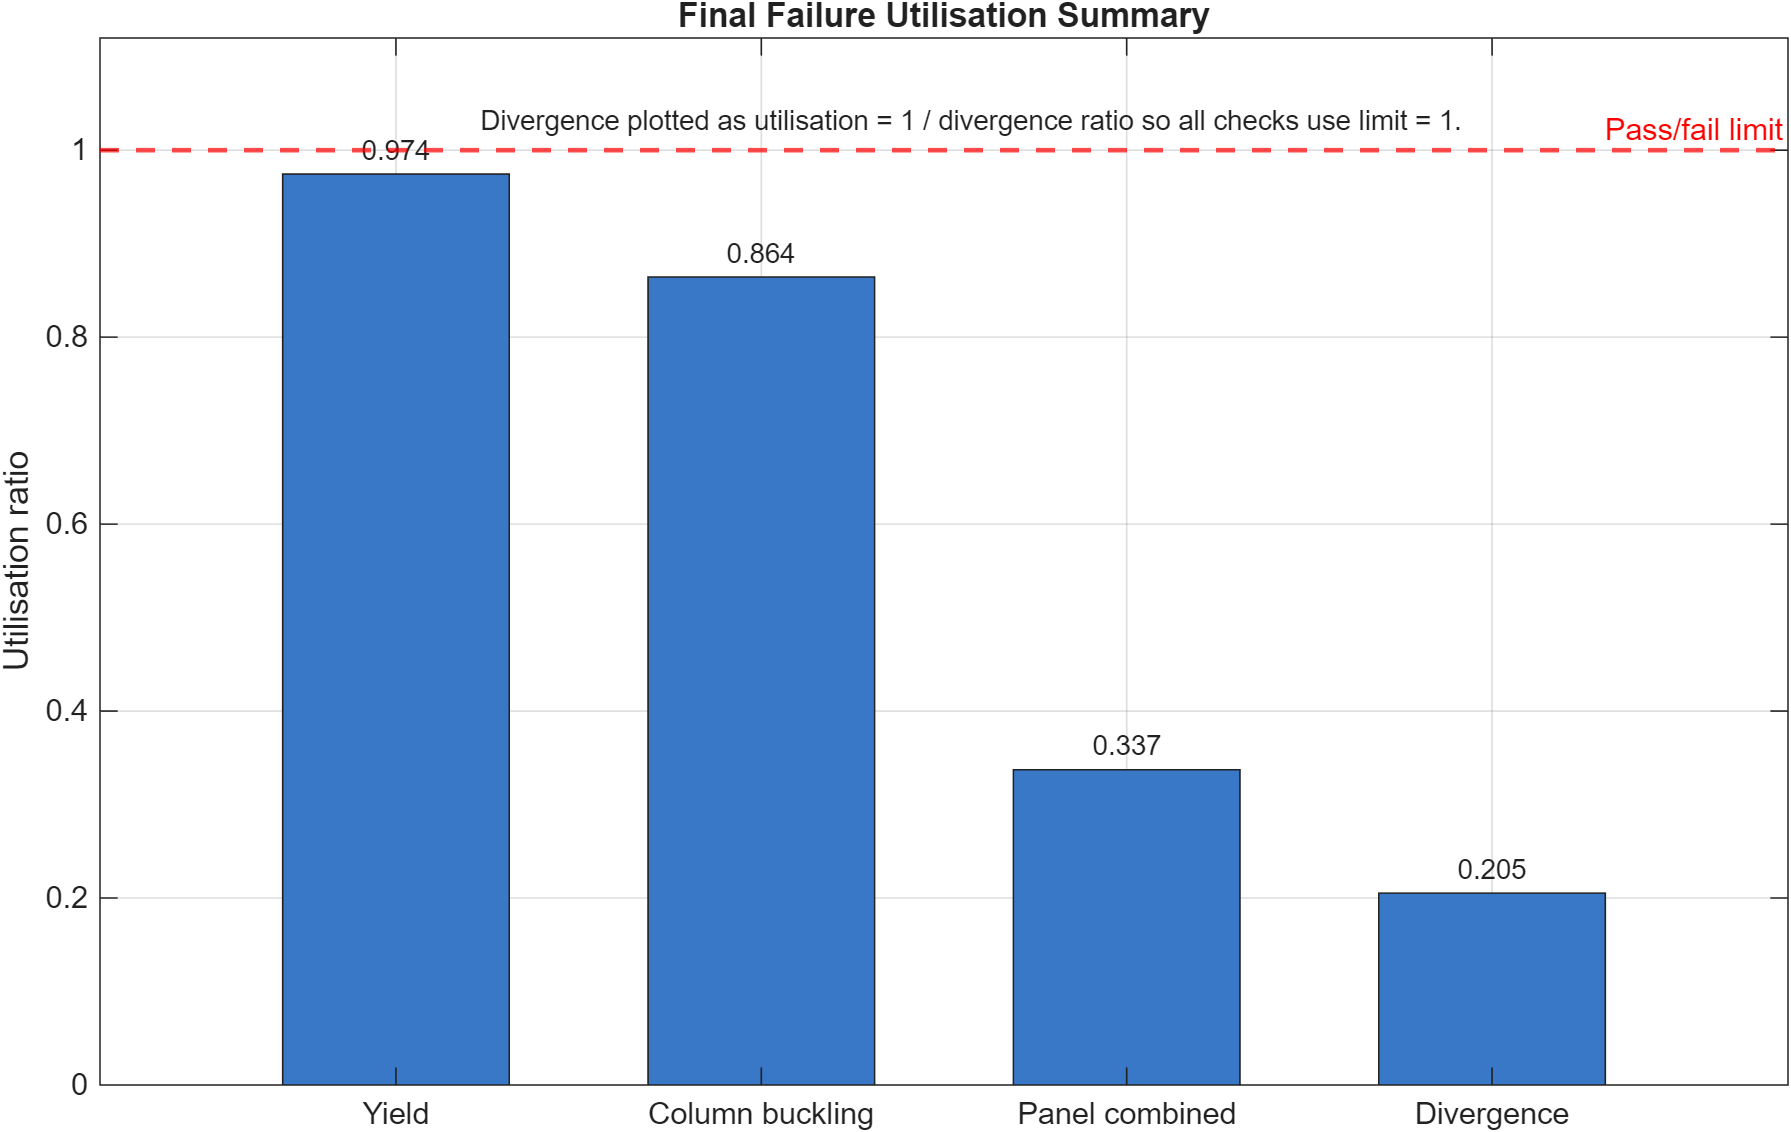
\includegraphics[width=0.78\linewidth]{final_failure_utilisation_bars.png}
\caption{Final failure utilisation bar chart.}
\label{fig:utilbars}
\end{figure}

\begin{figure}[H]
\centering
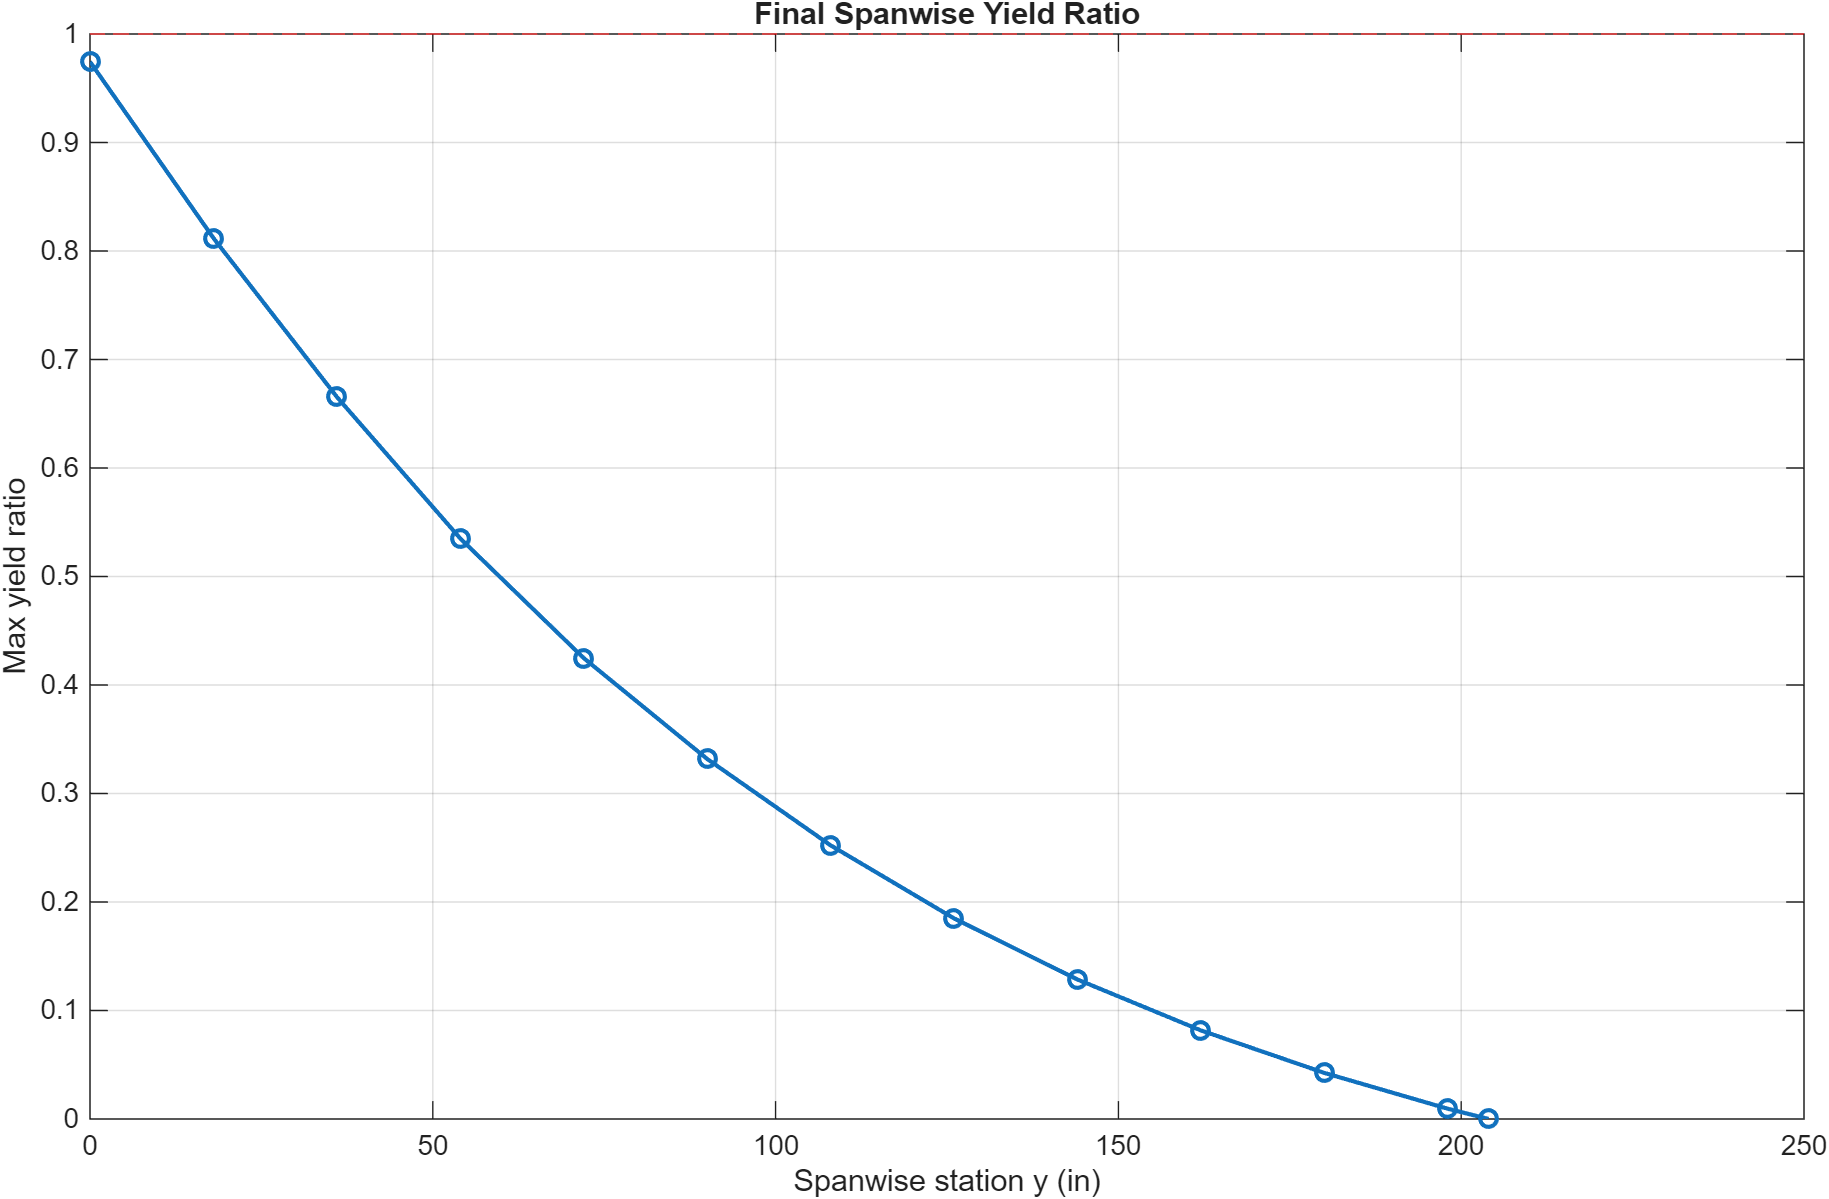
\includegraphics[width=0.82\linewidth]{final_spanwise_yield_ratio.png}
\caption{Maximum yield ratio by spanwise rib station.}
\label{fig:yieldspan}
\end{figure}

\begin{figure}[H]
\centering
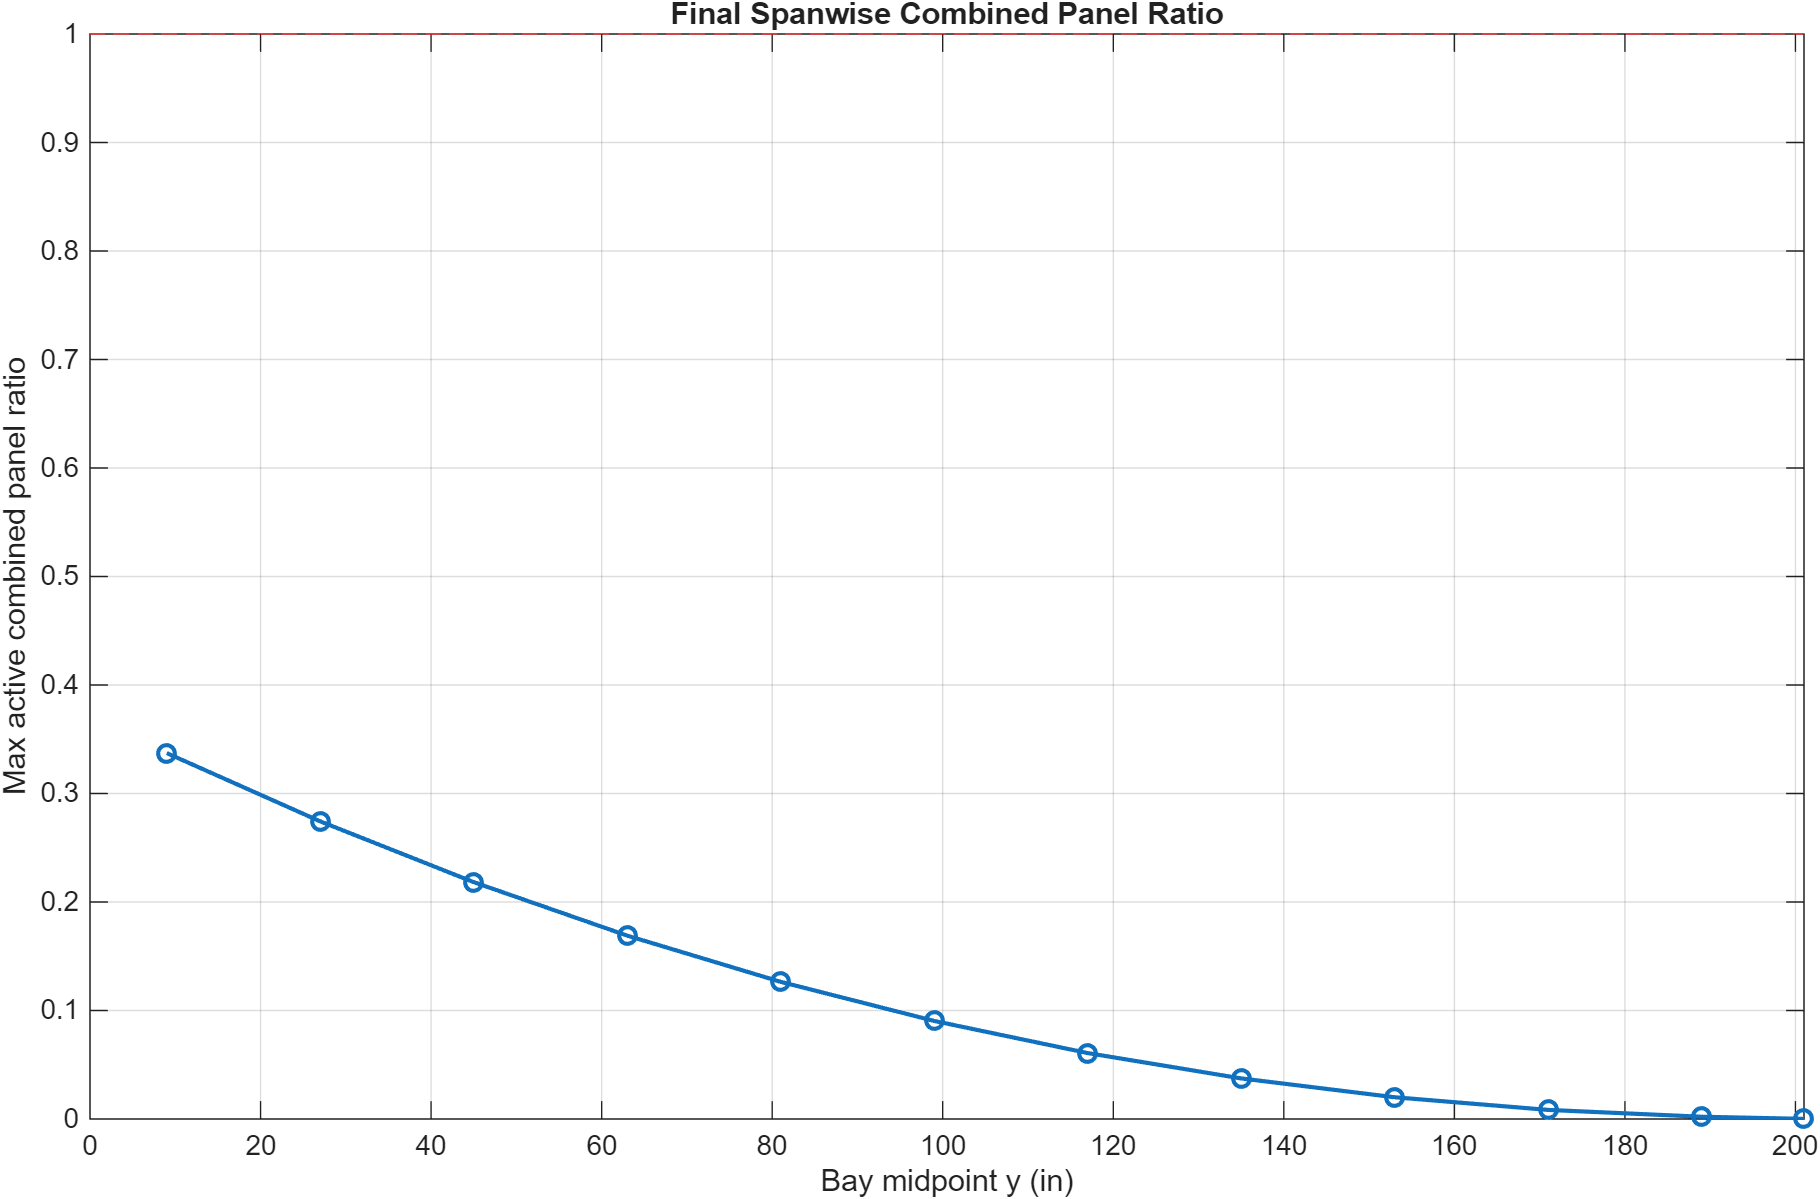
\includegraphics[width=0.82\linewidth]{final_spanwise_panel_combined_ratio.png}
\caption{Maximum active combined panel buckling ratio by bay.}
\label{fig:combinedspan}
\end{figure}

The stress-recovery plots in Figures~\ref{fig:bendingstress}, \ref{fig:panelshearstress}, and \ref{fig:shearflow} show the same root-dominated behaviour as the load distributions. These plots connect the applied load gradients to the final yield and panel buckling checks.

\begin{figure}[H]
\centering
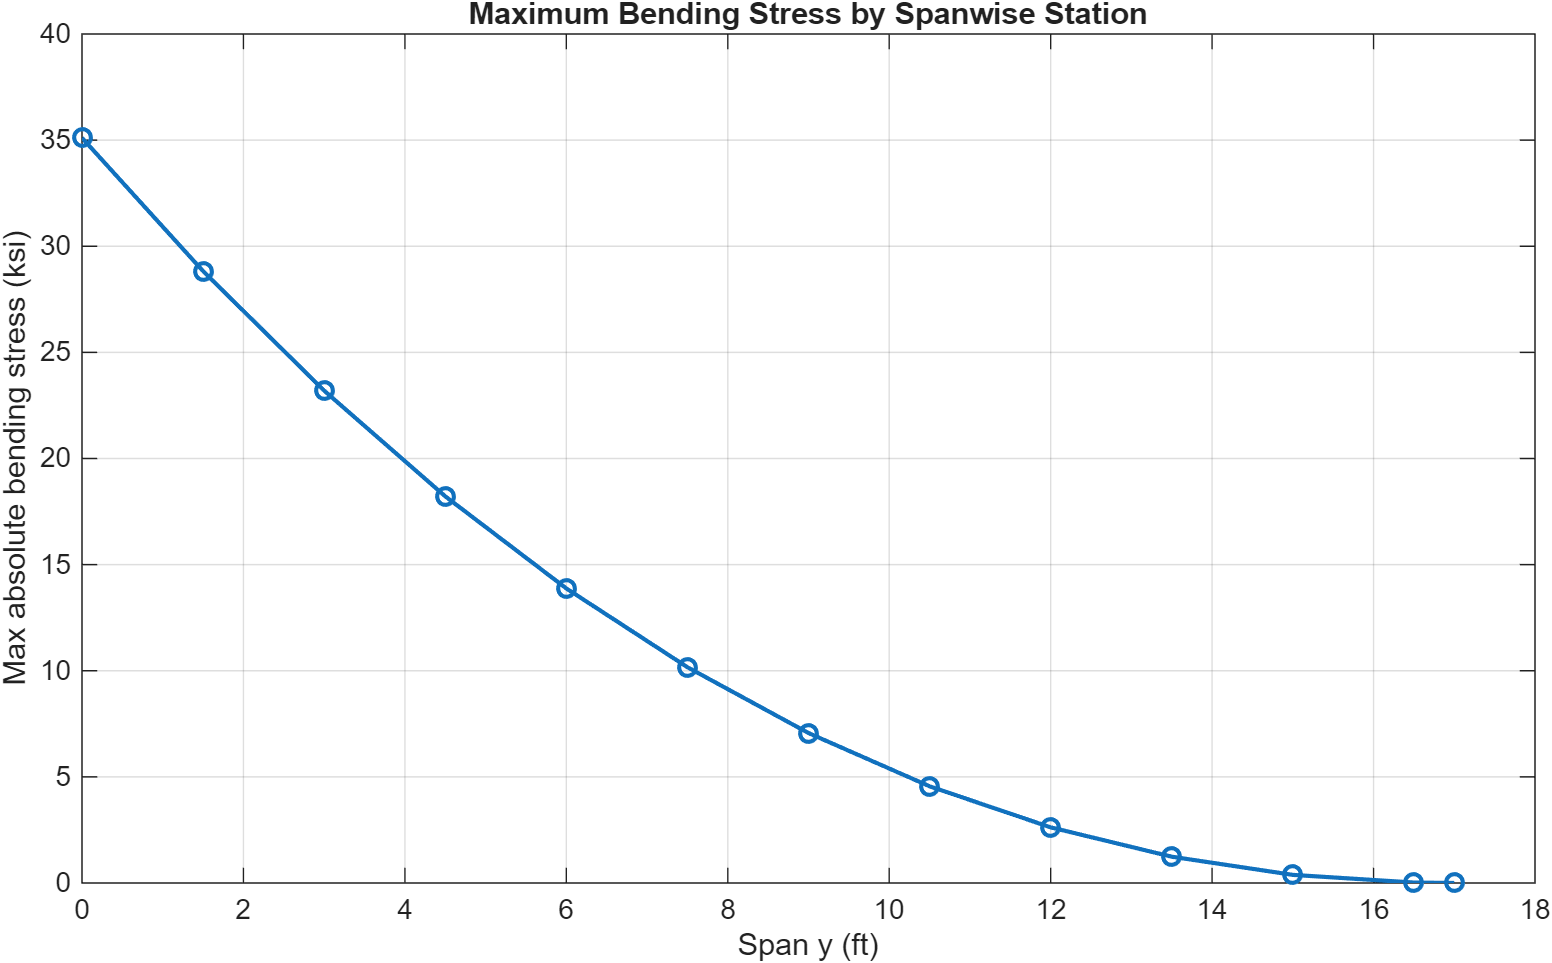
\includegraphics[width=0.82\linewidth]{final_spanwise_bending_stress.png}
\caption{Maximum absolute bending stress by spanwise station for the final design.}
\label{fig:bendingstress}
\end{figure}

\begin{figure}[H]
\centering
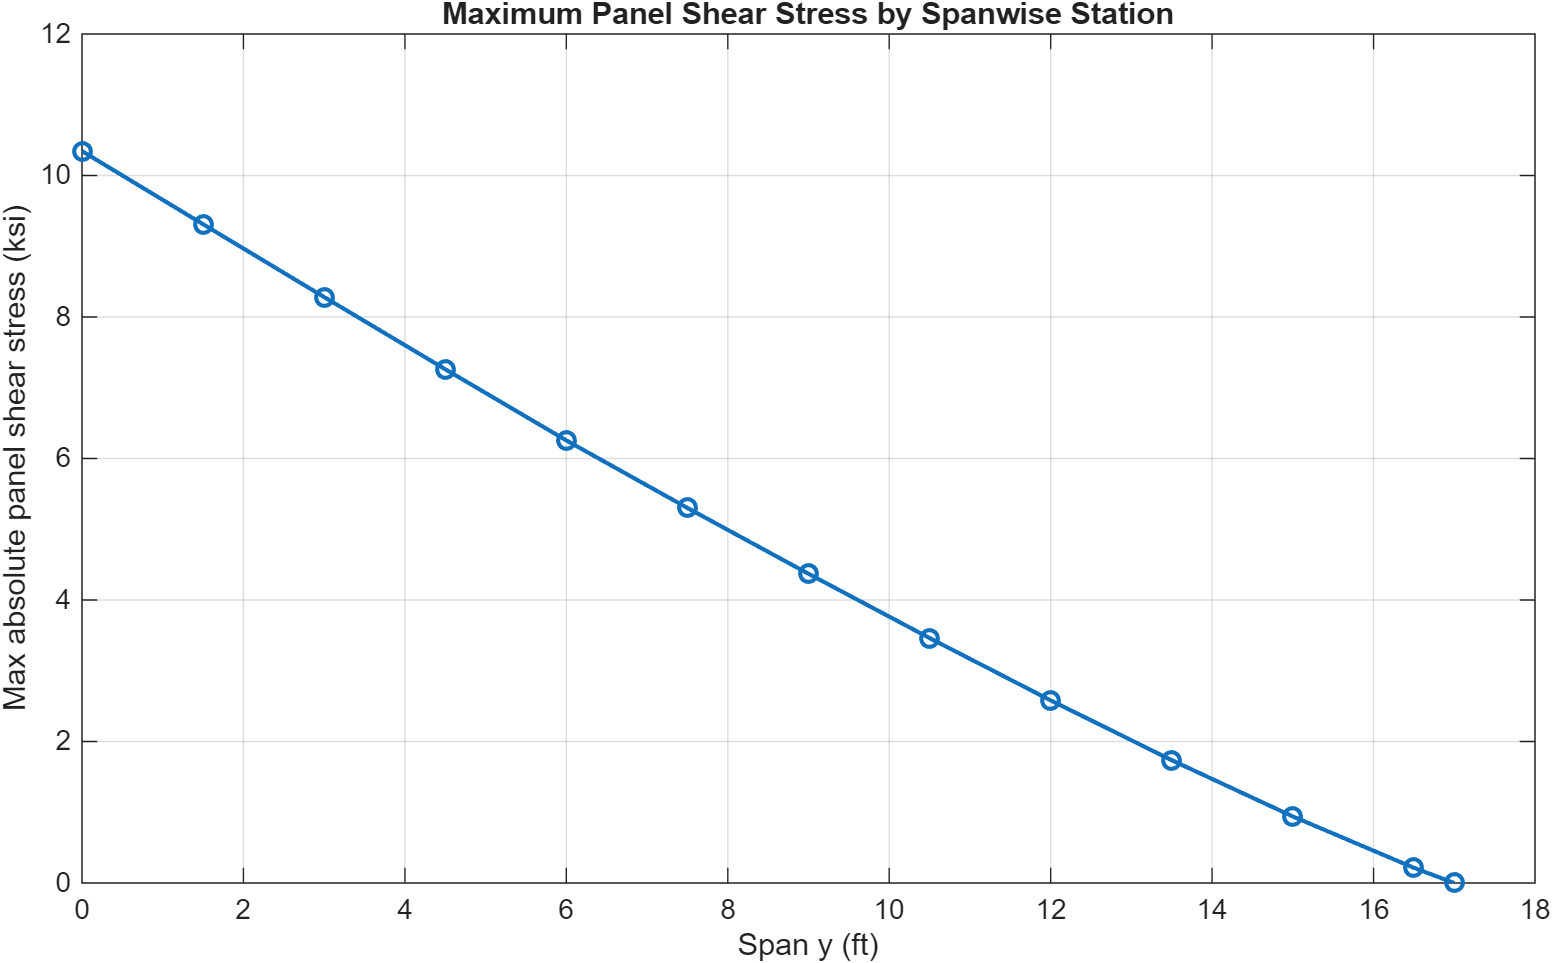
\includegraphics[width=0.82\linewidth]{final_spanwise_panel_shear_stress.png}
\caption{Maximum absolute panel shear stress by spanwise station for the final design.}
\label{fig:panelshearstress}
\end{figure}

\begin{figure}[H]
\centering
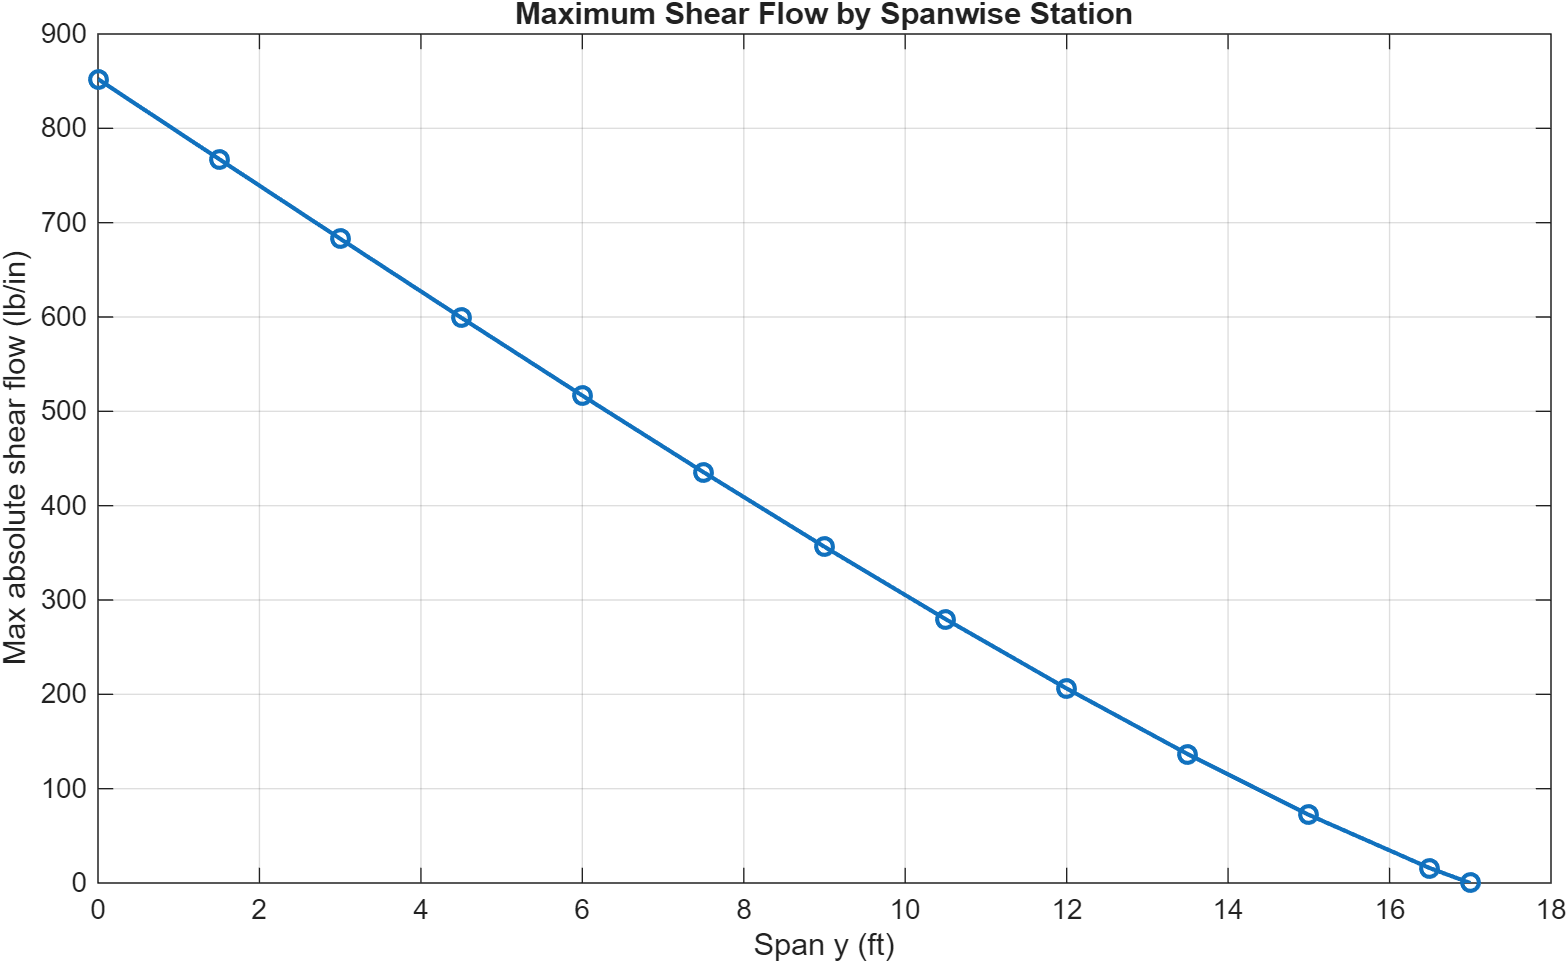
\includegraphics[width=0.82\linewidth]{final_spanwise_shear_flow.png}
\caption{Maximum absolute shear flow by spanwise station for the final design.}
\label{fig:shearflow}
\end{figure}

Figure~\ref{fig:bayutil3d} maps the active combined panel-buckling utilisation onto the wing-box bays. Each coloured spanwise segment corresponds to a bay between ribs, so the plot shows where the panel-buckling check is most active.

\begin{figure}[H]
\centering
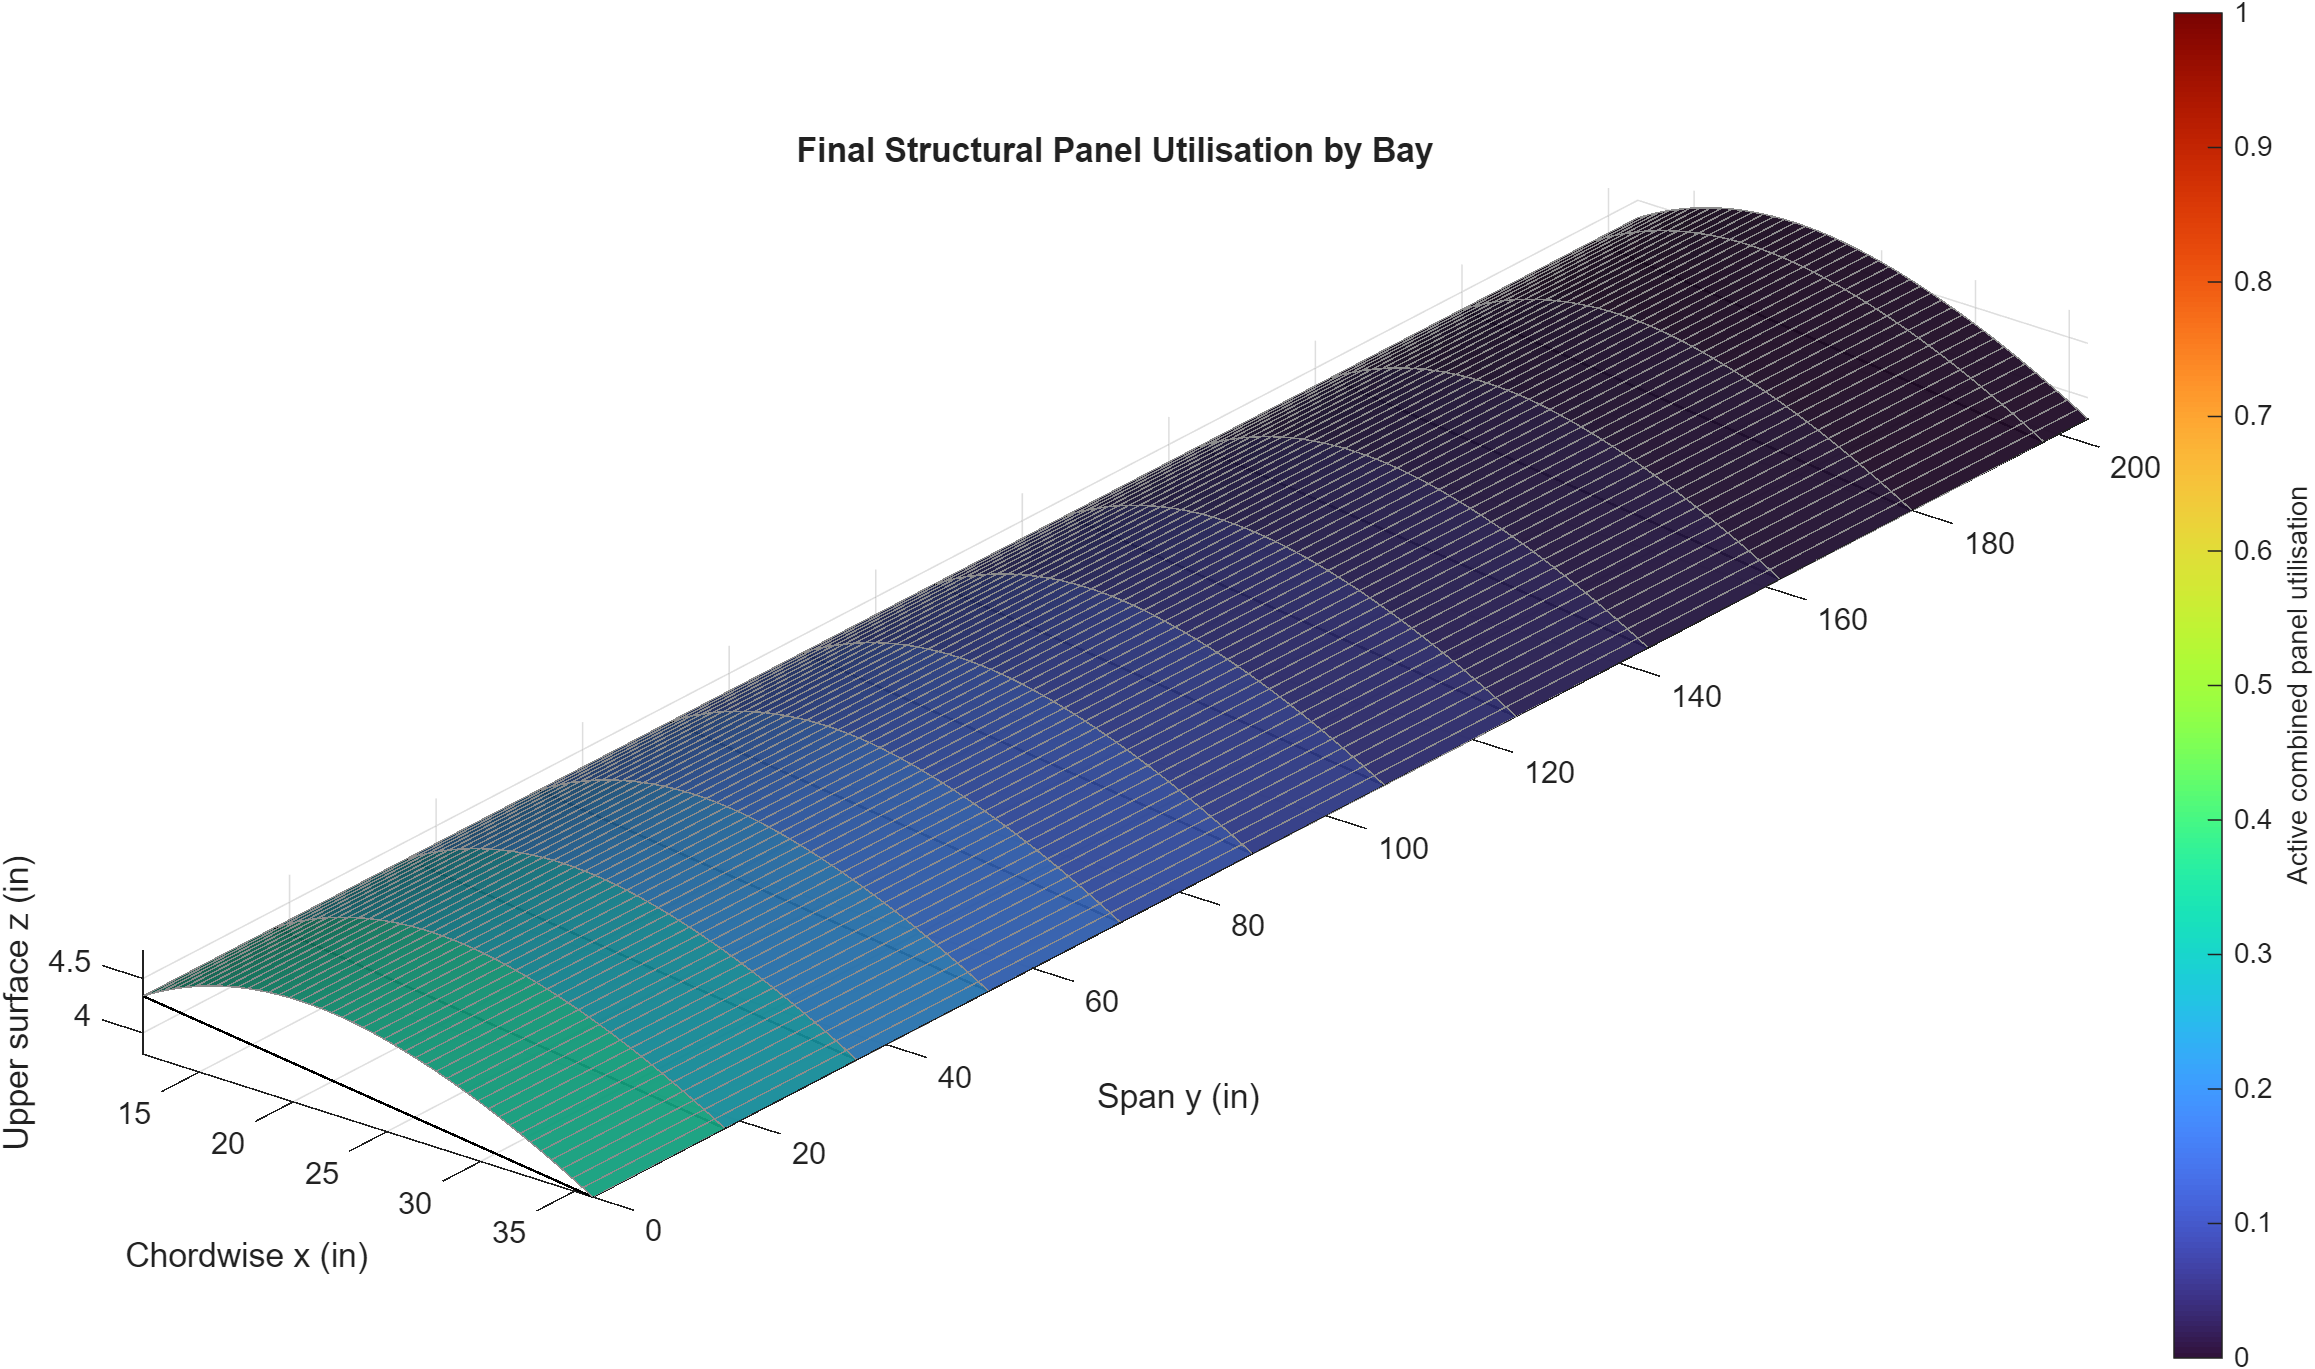
\includegraphics[width=0.88\linewidth]{final_wing_3d_structural_utilisation_by_bay.png}
\caption{Baywise active combined panel-buckling utilisation for the final design.}
\label{fig:bayutil3d}
\end{figure}

\section{Weight Breakdown}

The final total reported weight is approximately \SI{449.45}{lb}, including ribs and excluding miscellaneous detailed-design items. The geometric rib model gives \SI{0.8283}{lb} per rib and \SI{20.7067}{lb} fullspan for 25 ribs.

\begin{figure}[H]
\centering
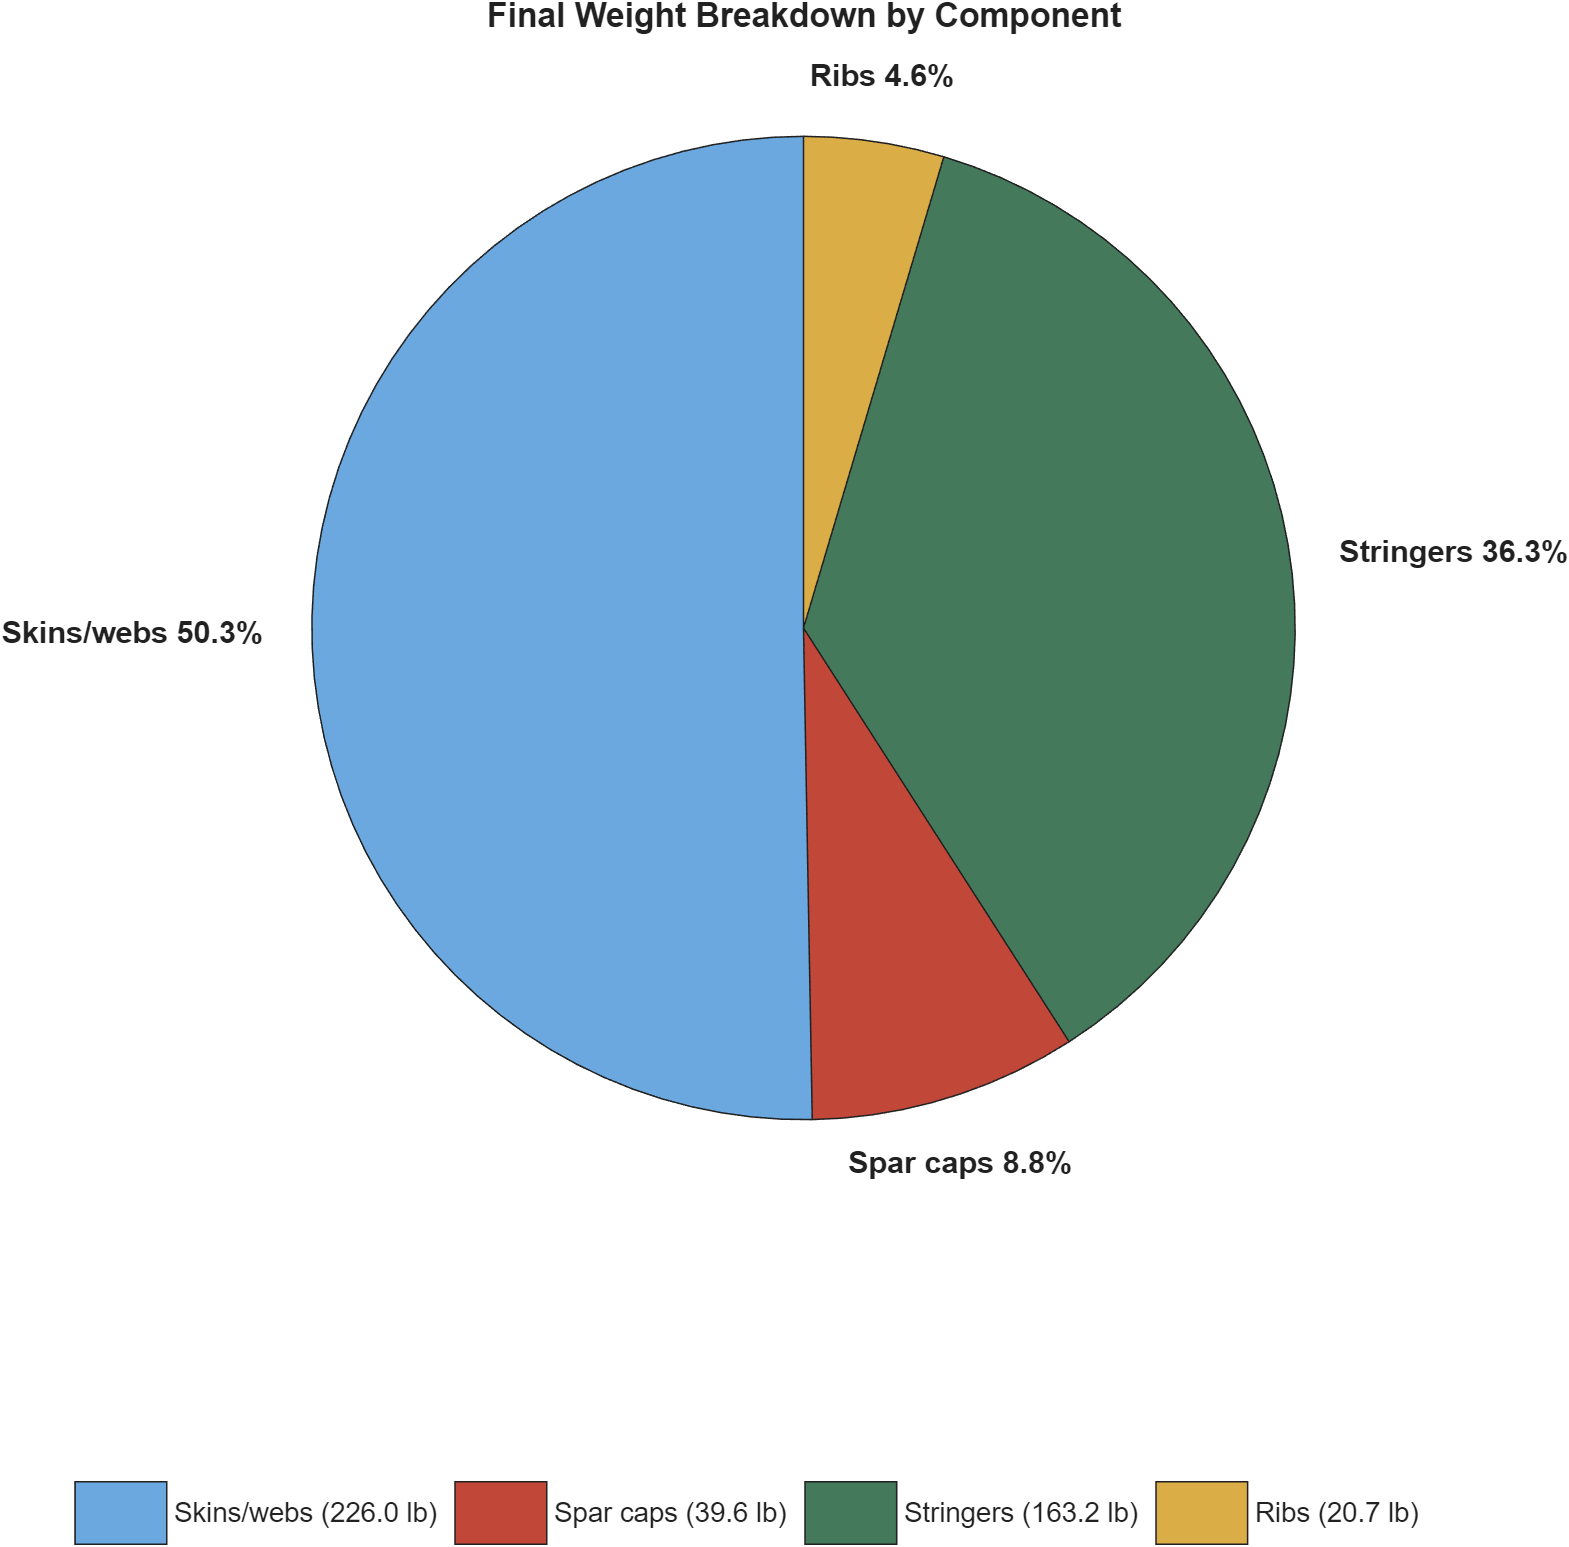
\includegraphics[width=0.68\linewidth]{final_weight_breakdown_pie.png}
\caption{Final structural weight fraction by major component group.}
\label{fig:weightpie}
\end{figure}

\begin{table}[H]
\centering
\caption{Final weight summary.}
\label{tab:weight}
\begin{tabular}{lc}
\toprule
Weight item & Fullspan weight (lb) \\
\midrule
Skins and webs & 225.9976 \\
Spar caps & 39.5597 \\
Stringers & 163.1837 \\
Ribs & 20.7067 \\
Total excluding ribs and misc. & 428.7410 \\
Total including ribs and excluding misc. & 449.4477 \\
\bottomrule
\end{tabular}
\end{table}

\section{Assumptions and Limitations}

The sizing model captures the primary structural components and stability drivers included in the model: skins, webs, spar caps, stringers, ribs, bending stress, shear flow, yield, Euler column buckling, panel buckling, combined panel loading, divergence, and geometric rib weight. Detailed-design items are outside the numerical scope of this work and could be added to extend the model.

\begin{itemize}
  \item Crippling is outside the numerical scope of the model and is not included in pass/fail.
  \item Detailed rib stress and rib buckling are outside scope; ribs are included in weight and define bay spacing.
  \item Fasteners, joints, doublers, paint, access panels, manufacturing allowances, fuel-system details, and other miscellaneous detailed-design items are excluded from the reported structural weight.
  \item Panel buckling coefficients are fixed estimates: $K_c=6$, $K_b=32$, and $K_s=8$.
  \item The spanwise section is treated as constant.
  \item Postbuckling and tension-field behaviour are not included.
\end{itemize}

\section{Conclusions}

The final adaptive Monte Carlo search identified a passing final wing-box candidate with a reported structural weight of approximately \SI{449.45}{lb}, including ribs and excluding miscellaneous detailed-design items. The design uses spars at $x/c=0.20$ and $x/c=0.60$, A3.10 Z-section stringers, and A3.13 T-section spar caps. The final design passes all implemented numerical checks, with yield ratio 0.9744, Euler column buckling ratio 0.8643, active combined panel buckling ratio 0.3372, and divergence ratio 4.8712. The final selected candidate should be understood as the lightest passing design found by the adaptive Monte Carlo search, subject to the stated assumptions and limitations.

\begin{thebibliography}{9}
\bibitem{far23} U.S. Code of Federal Regulations, Title 14, Part 23, \emph{Airworthiness Standards: Normal, Utility, Acrobatic, and Commuter Category Airplanes}, Sections 23.303, 23.333, 23.335, 23.337 and 23.341 (edition prior to Amendment 23-64).
\bibitem{bruhn} E.~F. Bruhn, \emph{Analysis and Design of Flight Vehicle Structures}, Jacobs Publishing, 1973.
\bibitem{megson} T.~H.~G. Megson, \emph{Aircraft Structures for Engineering Students}, Butterworth-Heinemann.
\bibitem{milhdbk5} U.S. Department of Defense, \emph{MIL-HDBK-5H: Metallic Materials and Elements for Aerospace Vehicle Structures}, 1998.
\bibitem{xfoil} M. Drela, \emph{XFOIL: An Analysis and Design System for Low Reynolds Number Airfoils}, Lecture Notes in Engineering, vol.~54, Springer, 1989.
\end{thebibliography}

\end{document}
